\section{Multivariable Differentiation}

So far we have worked only with functions in one variable (usually called $x$ or $t$).  In this chapter we will look at functions of multiple variables where those variables are allowed to be independent of one another.  The calculus of such functions is more complicated than the single variable case, and we will look at this in detail for functions of $2$ and $3$ variables.

\subsection{Functions of several variables}

  As always in this course, we will only deal with real functions of real variables.  Although we allow multiple variables, the value of the function will still be a single real number.

  \begin{definition}
    For a (non-zero) natural number $n$, a \emph{function $f$ of $n$ variables} is a function
      \[
        f \colon \mathbb{R}^n \longrightarrow \mathbb{R},
      \]
    or a function
      \[
        f \colon D \longrightarrow \mathbb{R},
      \]
    where $D \subset \mathbb{R}^n$.
  \end{definition}

  \subsubsection*{Remarks:}
    \begin{itemize}[topsep=0pt]
      \item We will focus on the cases when $n = 2$ and $n = 3$.
      \item As with the single variable case, we have to allow the domain to be a subset of $\mathbb{R}^n$, in case there are points at which the function is not defined (e.g. due to dividing by $0$, square roots of negatives, etc.).
      \item The codomain of our functions is always $\mathbb{R}$, \emph{not} $\mathbb{R}^n$.
    \end{itemize}

  \subsubsection*{Notation:}
    \begin{itemize}[topsep=0pt]
      \item For a function $f$ of $2$ variables, we write
        \[
          f(x, y)
        \]
      for the value of $f$ at the point $(x, y)$.
      \item Similarly, for a function $f$ of $3$ variables, we write
        \[
          f(x, y, z).
        \]
      \item For a function of $n$ variables, we write
        \[
          f(x_1, x_2, \dotsc, x_n).
        \]
    \end{itemize}

  \begin{examples}
  \
    \begin{enumerate}[topsep=0pt]
      \item Equation of a plane: linear expression in $x$ and $y$, e.g.
        \[
          f(x, y) = 3x - y + 2.
        \]
      \item Polynomials in $x$ and $y$, e.g.
        \[
          g(x, y) = x^3 + y^3 - 3x - 3y.
        \]
      \item We can include terms involving both $x$ and $y$:
        \[
          h(x, y) = x^2 + y^2 - \frac{1}{2}xy.
        \]
      \item A trigonometric example:
        \[
          k(x, y) = x\sin(y).
        \]
    \end{enumerate}
  \end{examples}

  We will use these examples throughout this chapter.  3D plots shown in the lecture.


\subsection{Partial derivatives}

  In this section we develop the tools for studying rates of change of functions of more than one variable.  As usual we do this using differentiation.

  We look at the two-variable case first (other cases are similar).  We are used to differentiating with respect to an independent variable, but now we have two independent variables, $x$ and $y$.

  Two possibilities:
    \begin{itemize}[topsep=0pt]
      \item Differentiate with respect to $x$; keep $y$ fixed.
      \item Differentiate with respect to $y$; keep $x$ fixed.
    \end{itemize}

  We can do either of these.  The derivatives we get are called \emph{partial derivatives}.

  \begin{definition}
    Given a function $f$ of two variables, if $(x_0, y_0)$ is a point in the domain of $f$, the \emph{partial derivative of $f$ with respect to $x$} is
    \[
      \frac{\partial f}{\partial x}(x_0, y_0) := \left. \frac{d}{dx}f(x, y_0) \right|_{x = x_0} = \lim_{\Delta x \rightarrow 0} \frac{f(x_0 + \Delta x, y_0) - f(x_0, y_0)}{\Delta x}.
    \]
    Similarly, the \emph{partial derivative of $f$ with respect to $y$} is
    \[
      \frac{\partial f}{\partial y}(x_0, y_0) := \left. \frac{d}{dx}f(x_0, y) \right|_{y = y_0} = \lim_{\Delta y \rightarrow 0} \frac{f(y_0, y_0 + \Delta y) - f(x_0, y_0)}{\Delta y}.
    \]
  \end{definition}

  This definition may look scary but the moral is fairly simple: if we fix $y$, $f$ becomes a function of $x$ only, and we can differentiate it with respect to $x$ in the usual way (and vice versa).

  \subsubsection*{Notation:}
  The partial derivatives are themselves functions of two variables $(x, y)$.  We write them either as
    \[
      \frac{\partial f}{\partial x}, \quad \frac{\partial f}{\partial y},
    \]
  or
    \[
      f_x(x, y), \quad f_y(x, y).
    \]
  The symbol $\partial$ is a stylised $d$ used mainly for partial derivatives.  It is derived from the Cyrillic alphabet.

  \subsubsection*{Interpretation}

  In the definition of $f_x(x, y)$, we treated $y$ as a constant (holding $y$ fixed) and differentiated with respect to $x$.  The act of fixing a value of $y$ corresponds to looking at a certain plane with an equation of the form $y = c$, a constant.  Such a plane intersects $z = f(x, y)$, as shown in figure (\ref{yfixed}).
%% \nextalt{Request description from lecturer or 3D object.}
%% \ifboolexpr{togl {clearprint} or togl {web}}
%% {
%%   \begin{figure}[H]
%%     \centering
%%     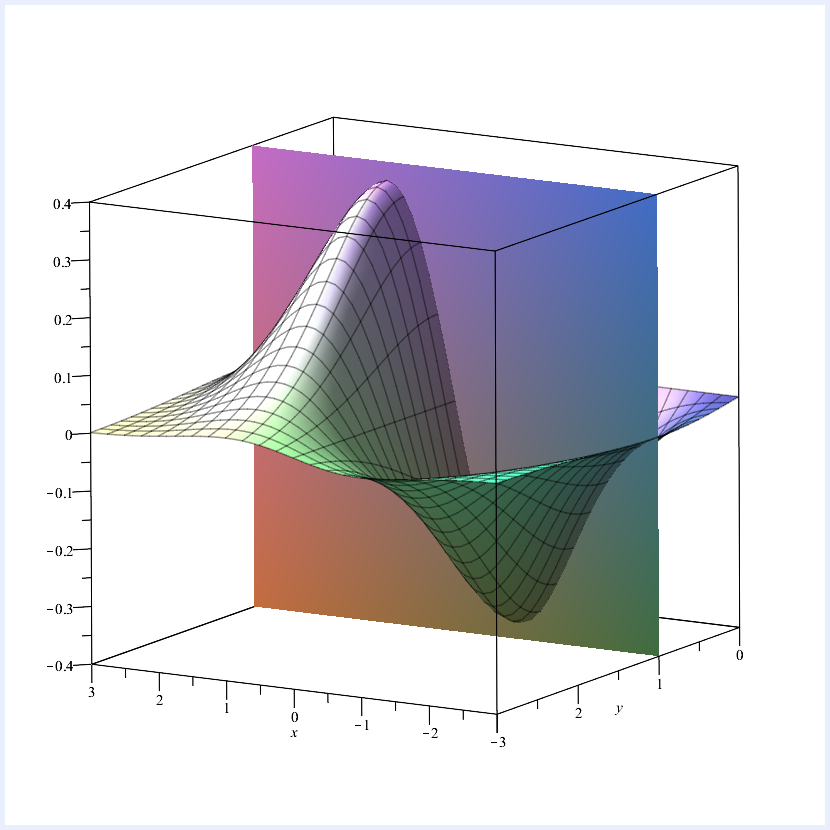
\includegraphics[width=0.75\textwidth]{yfixed.png}
%%     \caption{Plane intersecting $z = f(x, y)$}
%%     \label{yfixed}
%%   \end{figure}
%% }{
  \begin{figure}[H]
    \centering
    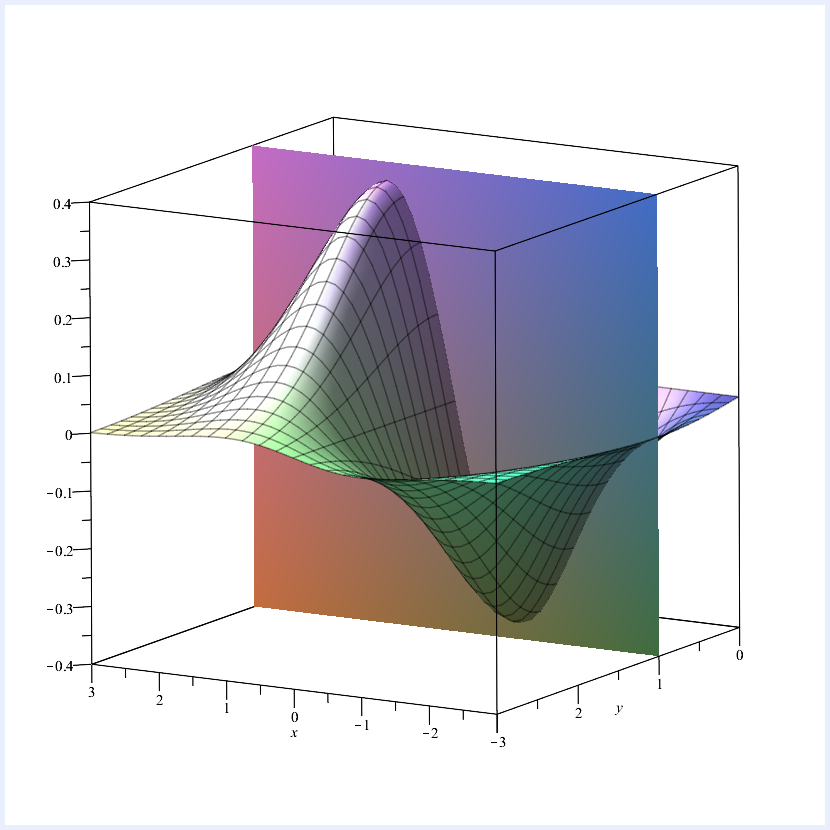
\includegraphics[width=0.51\textwidth]{yfixed.png}
    \caption{Plane intersecting $z = f(x, y)$}
    \label{yfixed}
  \end{figure}
%% }

  The intersection of the surface and the plane is a curve that depends on $x$.  The value of the partial derivative $f_x(x, y)$ at a particular point $(x, c)$ is the gradient of this curve for that particular $x$ value.  Similarly, for $f_y(x, y)$, the plane $x = c$ intersects $f(x, y)$ in a curve; $f_y(c, y)$ is the gradient of this curve for a given $y$ value.

  \begin{examples}
  \
    \begin{enumerate}
      \item $f(x, y) = 3x - y + 2$, then
        \[
          f_x(x, y) = 3, \quad f_y(x, y) = -1.
        \]
      \item $g(x, y) = x^3 + y^3 - 3x - 3y$, then
        \[
          g_x(x, y) = 3x^2 - 3, \quad g_y(x, y) = 3y^2 - 3.
        \]
      \item $h(x, y) = x^2 + y^2 - \frac{1}{2}xy$, then
        \[
          h_x(x, y) = 2x - \frac{1}{2}y, \quad h_y(x, y) = 2y - \frac{1}{2}x.
        \]
      \item $k(x, y) = x\sin(y)$, then
        \[
          k_x(x, y) = \sin(y), \quad k_y(x, y) = x\cos(y).
        \]
    \end{enumerate}
  \end{examples}

  \subsubsection*{Higher order partial derivatives}

  Partial derivatives are functions of two variables, so they have partial derivatives of their own.  The resulting functions are called \emph{second order partial derivatives}.  This is like the second derivative of a function of one variable, but now we have four possibilities:
    \[
      \frac{\partial^2 f}{\partial x^2} = \frac{\partial}{\partial x} \left( \frac{\partial f}{\partial x} \right) = f_{xx}, \quad\quad \frac{\partial^2 f}{\partial y^2} = \frac{\partial}{\partial y} \left( \frac{\partial f}{\partial y} \right) = f_{yy},
    \]
    \[
      \frac{\partial^2 f}{\partial y \partial x} = \frac{\partial}{\partial y} \left( \frac{\partial f}{\partial x} \right) = f_{xy}, \quad\quad \frac{\partial^2 f}{\partial x \partial y} = \frac{\partial}{\partial x} \left( \frac{\partial f}{\partial y} \right) = f_{yx}.
    \]
  The last two cases are called \emph{mixed second-order partial derivatives}.

  Similarly, third order, fourth order, etc. partial derivatives can be obtained by successive differentiation.

  % It's likely that there's not time to do all of these!  Possibly just do 2 and 3.
  \begin{examples}
  \
    \begin{enumerate}
      \item $f(x, y) = 3x - y + 2$, then
        \[
          f_{xx}(x, y) = 0, \quad f_{yy}(x, y) = 0,
        \]
        \[
          f_{xy}(x, y) = 0, \quad f_{yx}(x, y) = 0.
        \]
      \item $g(x, y) = x^3 + y^3 - 3x - 3y$, then
        \[
          g_{xx}(x, y) = 6x, \quad g_{yy}(x, y) = 6y,
        \]
        \[
          g_{xy}(x, y) = 0, \quad g_{yx}(x, y) = 0,
        \]
      \item $h(x, y) = x^2 + y^2 - \frac{1}{2}xy$, then
        \[
          h_{xx}(x, y) = 2, \quad h_{yy}(x, y) = 2,
        \]
        \[
          h_{xy}(x, y) = -\frac{1}{2}, \quad h_{yx}(x, y) = -\frac{1}{2}.
        \]
      \item $k(x, y) = x\sin(y)$, then
        \[
          k_{xx}(x, y) = 0, \quad k_{yy}(x, y) = -x\sin(y),
        \]
        \[
          k_{xy}(x, y) = \cos(y), \quad k_{yx}(x, y) = \cos(y).
        \]
    \end{enumerate}
  \end{examples}

  \subsubsection*{Equality of mixed partials}

  In the examples, the two mixed partials were equal.  This is true in general.

  \begin{theorem}[Clairaut's Theorem]  \label{thm:mixedpartials}
    Let $f$ be a function of two variables.  If $\dfrac{\partial^2 f}{\partial y \partial x}$ and $\dfrac{\partial^2 f}{\partial x \partial y}$ are continuous at a point $(a, b)$, then
    \[
      \dfrac{\partial^2 f}{\partial y \partial x}(a, b) = \dfrac{\partial^2 f}{\partial x \partial y}(a, b).
    \]
  \end{theorem}

  %\emph{Note:} An open disc is a circular region of the $(x, y)$-plane, not including the boundary of the circle.  Open discs are important in analysis.

  See Analysis 2B for a proof.	A version of Theorem~\ref{thm:mixedpartials} also holds in the $n$-variable case for $n > 2$.


\subsection{Critical points}
  % This section is currently probably too verbose.
  % I may also need to cut back on the environments -- there are a lot more than in the earlier sections and their use probably doesn't contribute much.

  In the one-variable case we can use the derivative of a function to find its critical points: maxima, minima, and points of inflection.  We can do something similar for functions of two variables, using partial derivatives.

  First, we want to know what kind of features we're trying to identify.  As in the one-variable case, we have \emph{maxima} and \emph{minima}, which can be either absolute (aka global) or relative (aka local) (see figure (\ref{absmaxmin})).

%% \nextalt{Request description from lecturer or 3D object.}
%% \ifboolexpr{togl {clearprint} or togl {web}}
%% {
%% \begin{figure}[!htbp]
%% \centering
%%  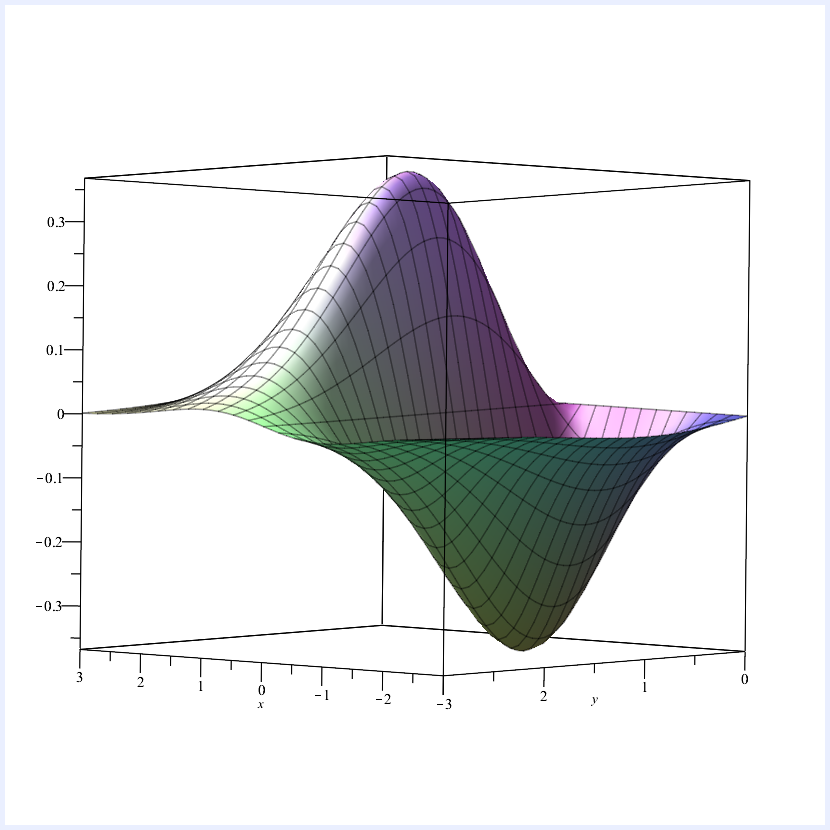
\includegraphics[width=0.75\textwidth]{maxandmin.png}
%% \caption{A function with an absolute maximum and absolute minimum.}
%% \label{absmaxmin}
%% \end{figure}
%% }{
\begin{figure}[!htbp]
\centering
 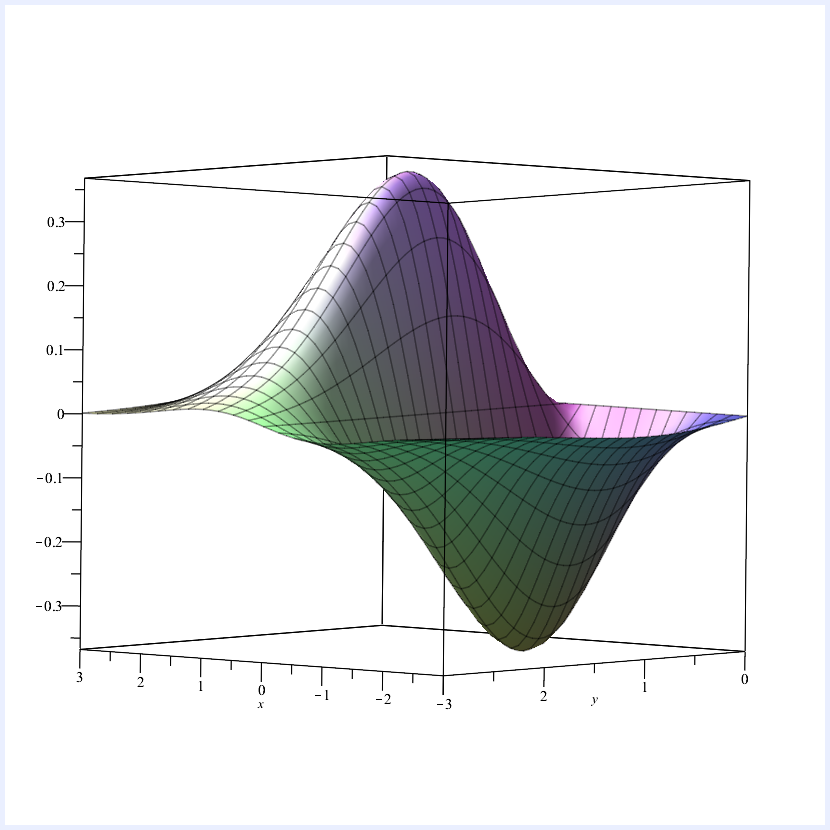
\includegraphics[width=0.55\textwidth]{maxandmin.png}
\caption{A function with an absolute maximum and absolute minimum.}
\label{absmaxmin}
\end{figure}
%% }

  The definitions of global maxima and minima are straightforward:

  \begin{definition}
    A function $f$ of two variables is said to have an \emph{absolute maximum} at $(x_0, y_0)$ if $f(x_0, y_0) \geq f(x, y)$ for all $(x, y)$.

    A function $f$ of two variables is said to have an \emph{absolute minimum} at $(x_0, y_0)$ if $f(x_0, y_0) \leq f(x, y)$ for all $(x, y)$.
  \end{definition}

\newpage

  The definitions of the relative versions are a bit fiddly (see figure (\ref{relmaxnabs})):

  \begin{definition}
    A function $f$ of two variables is said to have a \emph{relative maximum} at $(x_0, y_0)$ if there is a disc centred at $(x_0, y_0)$ such that $f(x_0, y_0) \geq f(x, y)$ for all $(x, y)$ inside the disc.

    A function $f$ of two variables is said to have a \emph{relative minimum} at $(x_0, y_0)$ if there is a disc centred at $(x_0, y_0)$ such that $f(x_0, y_0) \leq f(x, y)$ for all $(x, y)$ inside the disc.
  \end{definition}

%% \nextalt{Request description from lecturer or 3D object.}
%% \ifboolexpr{togl {clearprint} or togl {web}}
%% {
%% \begin{figure}[H]
%% \centering
%%  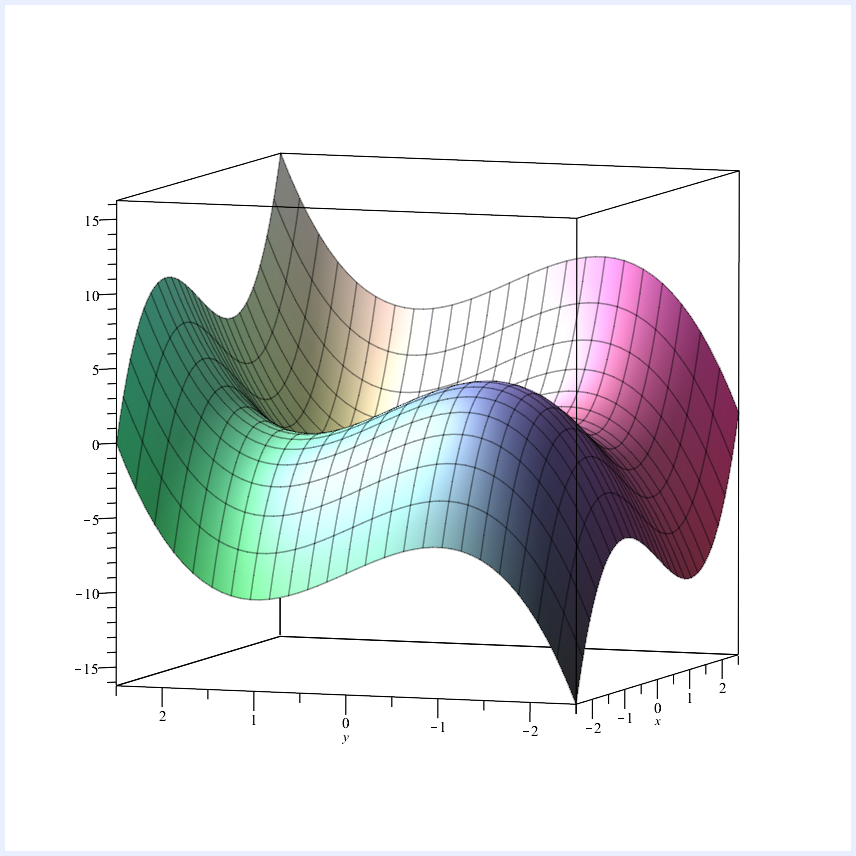
\includegraphics[width=0.75\textwidth]{relativemax.png}
%% \caption{A function with a relative maximum that is not absolute.}
%% \label{relmaxnabs}
%% \end{figure}
%% }{
\begin{figure}[H]
\centering
 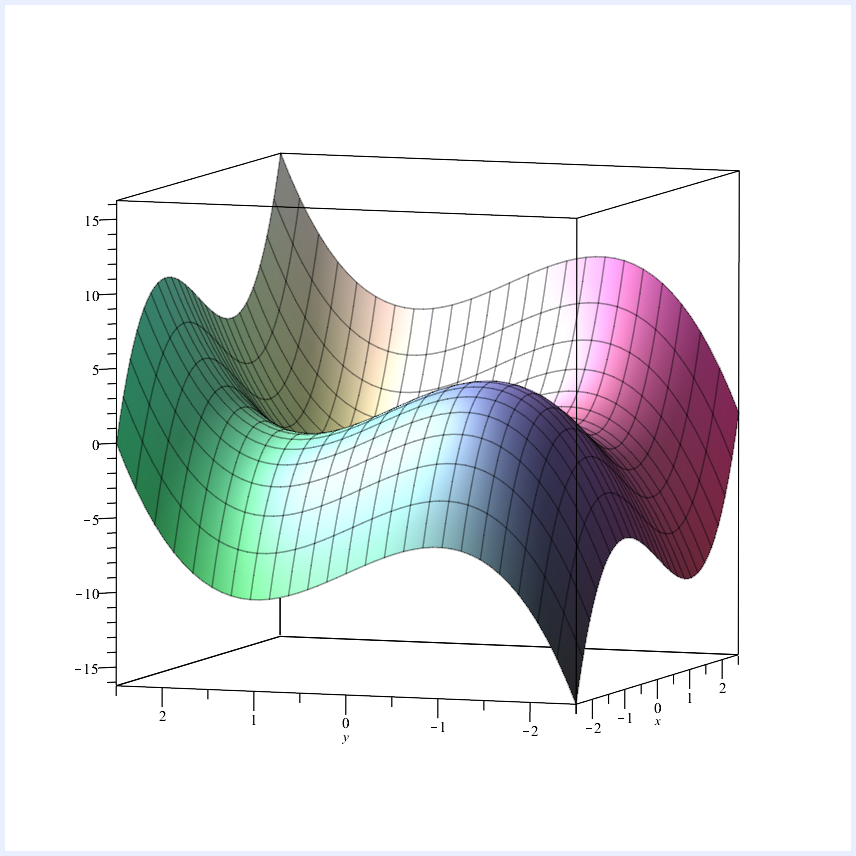
\includegraphics[width=0.55\textwidth]{relativemax.png}
\caption{A function with a relative maximum that is not absolute.}
\label{relmaxnabs}
\end{figure}
%%}

  % Technical definitions of maxima and minima.
  % Do I really need these?

  Collectively, maxima and minima are called \emph{extrema} (singular: extremum).  We can use partial derivatives to find most extrema (except for those on the boundaries of the domain), due to the following result:

  \begin{theorem}
    If $f$ has a relative extremum at $(x_0, y_0)$, and if the partial derivatives of $f$ exist at $(x_0, y_0)$, then
      \[
        \frac{\partial f}{\partial x}(x_0, y_0) = 0, \quad \frac{\partial f}{\partial y}(x_0, y_0) = 0.
      \]
  \end{theorem}

  The converse is not necessarily true: if the partial derivatives at a point are both $0$, that point is not guaranteed to be a relative extremum.

  \begin{definition}
    A point $(x_0, y_0)$ in the domain of a function $f(x, y)$ is called a \emph{critical point} if
      \[
        \frac{\partial f}{\partial x}(x_0, y_0) = 0, \quad \frac{\partial f}{\partial y}(x_0, y_0) = 0,
      \]
    or if one or both partial derivatives do not exist at $(x_0, y_0)$.
  \end{definition}

  As in the one-variable case, not all critical points are extrema.  A critical point that is not an extremum is called a \emph{saddle point} (figure (\ref{saddle})):

%% \nextalt{Request description from lecturer or 3D object.}
%% \ifboolexpr{togl {clearprint} or togl {web}}
%% {
%%   \begin{figure}[H]
%%     \centering
%%     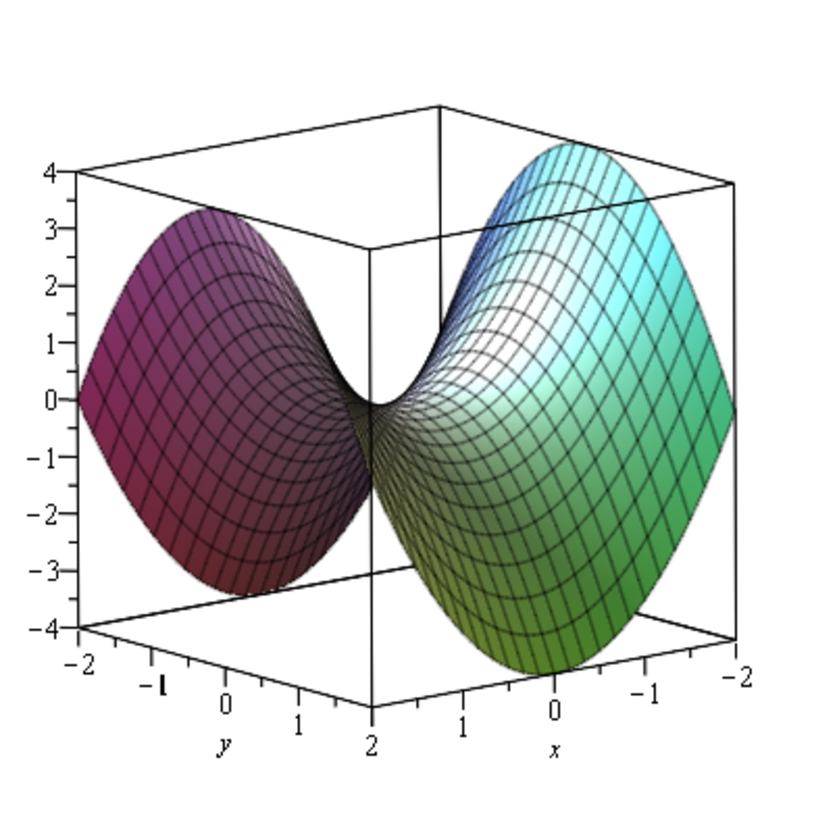
\includegraphics[width=0.75\textwidth]{paraboloid.pdf}
%%     \caption{Saddle point}
%%     \label{saddle}
%%   \end{figure}
%%   % Also, Pringles
%% }{
  \begin{figure}[H]
    \centering
    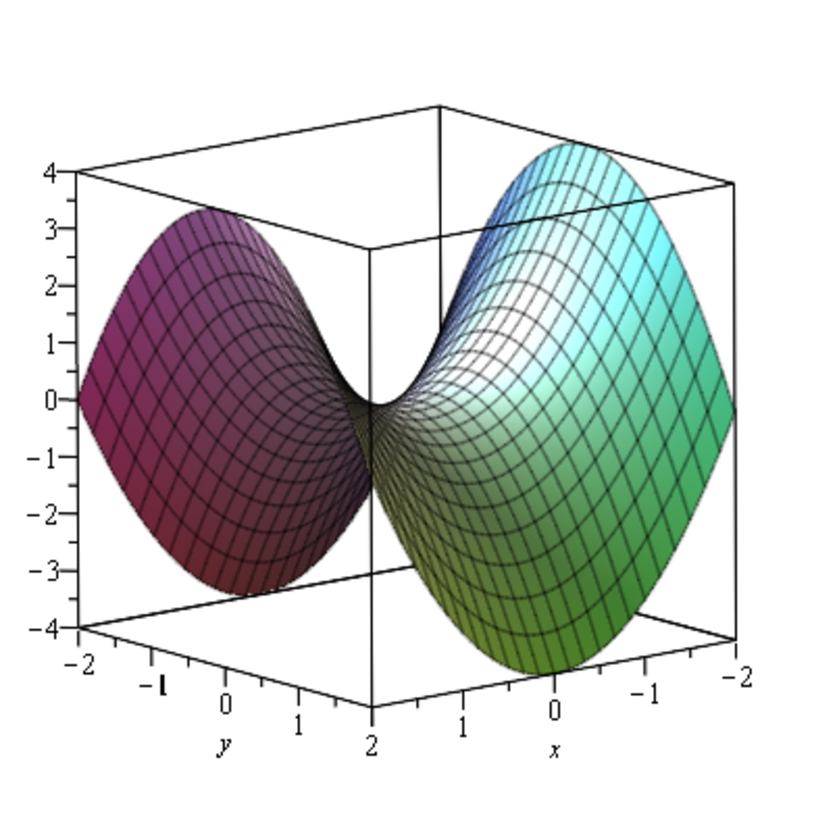
\includegraphics[width=0.6\textwidth]{paraboloid.pdf}
    \caption{Saddle point}
    \label{saddle}
  \end{figure}
  % Also, Pringles
%%}

  How do we tell if a critical point is an extremum?

  \begin{theorem}[Second Partials Test]
    Let $f$ be a function of two variables with continuous second-order partial derivatives in some disc centred at a critical point $(x_0, y_0)$, and let
    \[
      D = f_{xx}(x_0, y_0)f_{yy}(x_0, y_0) - f_{xy}(x_0, y_0)^2.
    \]
    \begin{enumerate}[label=(\alph*)]
      \item If $D > 0$ and $f_{xx}(x_0, y_0) > 0$, then $(x_0, y_0)$ is a relative minimum.
      \item If $D > 0$ and $f_{xx}(x_0, y_0) < 0$, then $(x_0, y_0)$ is a relative maximum.
      \item If $D < 0$, then $(x_0, y_0)$ is a saddle point.
      \item If $D = 0$, no conclusion can be drawn.
    \end{enumerate}
  \end{theorem}
	
	For a proof, see Analysis 2B; here we simply give some informal justification.
	
	Compare this with the one-variable version: suppose $f(x)$ has a critical point at $x_0$.  If $f''(x_0) < 0$, the gradient is decreasing as $x$ increases, so $x_0$ is a relative maximum.  Similarly, if $f''(x_0) > 0$, the gradient is increasing as $x$ increases, so $x_0$ is a relative minimum.
	
	Now consider the two-variable case.  If $D > 0$, then $f_{xx}$ and $f_{yy}$ have the same sign at $(x_0, y_0)$, and $f_{xy}$ is comparatively small, indicating little interaction between the two variables.  Thus, similar to the one-variable case, either $f_{xx}$, $f_{yy} < 0$ and the critical point is a relative maximum, or $f_{xx}$, $f_{yy} > 0$ and it is a relative minimum.
	
	If $D < 0$, then either $f_{xx}$ and $f_{yy}$ have different signs at $(x_0, y_0)$, or $f_{xy}$ is comparatively large and there is a lot of interaction between variables (or both).  Either of these possibilities leads to a saddle point.

  \begin{note}
    The $D$ stands for \emph{determinant}, so-called since it determines the nature of critical point.  It can also be expressed as the determinant of a matrix whose entries are the second order partials.
  \end{note}
  % Might be worth deformalising this, getting rid of most environments and making it notier/chattier.

  \begin{example}
    Recall the function $g(x, y) = x^3 + y^3 - 3x - 3y$.  The critical points occur when
      \[
        g_x(x, y) = 3x^2 - 3 = 0, \quad g_y(x, y) = 3y^3 - 3 = 0,
      \]
    i.e. when
      \[
        x^2 = 1, y^2 = 1.
      \]
    So the critical points are
      \[
        (1, 1), (-1, 1), (1, -1), (-1, -1).
      \]
    We use the second partial test:
      \[
        D = g_{xx}(x, y)g_{yy}(x, y) - g_{xy}(x, y)^2 = 6x \times 6y - 0 \times 0 = 36xy,
      \]
    so
      \begin{itemize}
        \item at $(1, 1)$, $D > 0$ and $g_{xx}(1, 1) > 0$, so $(1, 1)$ is a relative minimum;
        \item at $(-1, 1)$, $D < 0$, so $(-1, 1)$ is a saddle point;
        \item at $(1, -1)$, $D < 0$, so $(1, -1)$ is a saddle point;
        \item at $(-1, -1)$, $D > 0$, $g_{xx}(-1, -1) < 0$, so $(-1, -1)$ is a relative maximum.
      \end{itemize}
  \end{example}


  \subsection{Chain rules}

  As in the one-variable case, there are chain rules for differentiating composite functions of several variables.  There are various cases.

  \subsubsection*{Variables depend on $t$}

  The simplest case is the following:  let $f$ be a differentiable function of two variables $x$ and $y$, where $x = x(t)$, $y = y(t)$ are differentiable functions of $t$.  Then $f(x(t), y(t))$ is a differentiable function of $t$, and
    \[
      \frac{df}{dt} = \frac{\partial f}{\partial x}\frac{dx}{dt} + \frac{\partial f}{\partial y}\frac{dy}{dt}.
    \]

  The three-variable version is similar: let $f$ be a differentiable function of three variables $x$, $y$ and $z$, where $x = x(t)$, $y = y(t)$, $z = z(t)$ are differentiable functions of $t$.  Then $f(x(t), y(t), z(t))$ is a differentiable function of $t$, and
    \[
      \frac{df}{dt} = \frac{\partial f}{\partial x}\frac{dx}{dt} + \frac{\partial f}{\partial y}\frac{dy}{dt} + \frac{\partial f}{\partial z}\frac{dz}{dt}.
    \]

  \begin{examples} \
    \begin{enumerate}
      \item We begin with a simple example where we can easily find the answer directly.  Let
        \[
          z = x^2 y, \quad x = t^3, \quad y = t^2.
        \]
      Then, by the chain rule,
        \begin{align*}
          \frac{dz}{dt} & = \frac{\partial z}{\partial x}\frac{dx}{dt} + \frac{\partial z}{\partial y}\frac{dy}{dt}  \\
          & = 2xy \times 3t^2 + x^2 \times 2t  \\
          & = (2t^5)(3t^2) + (t^6)(2t)  \\
          & = 6t^7 + 2t^7 = 8t^7.
        \end{align*}
      We can check this directly by writing $z$ purely in terms of $t$:
        \[
          z = x^2 y = t^6 \times t^2 = t^8,
        \]
      so
        \[
          \frac{dz}{dt} = 8t^7.
        \]
      \item Let
        \[
          z = \sqrt{y^2 - xy}, \quad x = \cos(\theta), \quad y = \sin(\theta).
        \]
      Find the value of $\displaystyle \frac{dz}{d\theta}$ at $\displaystyle \theta = \frac{\pi}{2}$.

      By the chain rule,
        \begin{align*}
          \frac{dz}{d\theta} & = \frac{\partial z}{\partial x}\frac{dx}{d\theta} + \frac{\partial z}{\partial y}\frac{dy}{d\theta}  \\
          & = \frac{-y}{2\sqrt{y^2 - xy}} \times (-\sin(\theta)) + \frac{2y - x}{2\sqrt{y^2 - xy}} \times \cos(\theta).
        \end{align*}
      Now, at $\displaystyle \theta = \frac{\pi}{2}$,
        \[
          x = \cos\left(\frac{\pi}{2}\right) = 0, \quad y = \sin\left(\frac{\pi}{2}\right) = 1,
        \]
      so
        \[
          \frac{dz}{d\theta}\left(\frac{\pi}{2}\right) = \frac{-1}{2\sqrt{1 - 0}}\times(-1) + \frac{2 - 0}{2\sqrt{1 - 0}}\times 0 = \frac{1}{2}.
        \]
    \end{enumerate}
  \end{examples}

  \subsubsection*{Some useful applications of the chain rule}

  \begin{enumerate}
    \item Deriving rules of differentiation, e.g. the Product Rule.  What is
      \[
        \frac{d}{dx}(u(x)v(x)) \text{?}
      \]
      We can think of this as
      \[
        f(u, v) = uv
      \]
      where $u = u(x)$, $v = v(x)$ are functions of $x$.  By the chain rule
      \[
        \frac{df}{dx} = \frac{\partial f}{\partial u}\frac{du}{dx} + \frac{\partial f}{\partial v}\frac{dv}{dx}.
      \]
      We have
      \[
        \frac{\partial f}{\partial u} = v, \quad \frac{du}{dx} = u'(x), \quad \frac{\partial f}{\partial v} = u, \quad \frac{dv}{dx} = v'(x),
      \]
      so
      \[
        \frac{df}{dx} = v(x)u'(x) + u(x)v'(x).
      \]
      Similarly, we can derive the quotient rule.

      We can also derive a rule for differentiating functions of the form
        \[
          f(x) = u(x)^{v(x)}.
        \]
      (See Worksheet 7, exercise 5.)
      % This is likely to change!
    \item Differentiating $f(x, y)$, where $y$ depends on $x$.

    Think of this as $f(u, y)$, where
      \[
        u = u(x) = x, \quad y = y(x).
      \]
    Then $\displaystyle \frac{du}{dx} = 1$, so by the chain rule
      \[
        \frac{df}{dx} = \frac{\partial f}{\partial u}\frac{du}{dx} + \frac{\partial f}{\partial y}\frac{dy}{dx} = \frac{\partial f}{\partial x} + \frac{\partial f}{\partial y}\frac{dy}{dx}.
      \]
  \end{enumerate}


  \subsubsection*{Variables depend on $u$ and $v$}

  In the next case, the variables are themselves functions of two variables, $u$ and $v$.

  Let $f$ be a differentiable function of two variables $x$ and $y$, where
    \[
      x = x(u, v), \quad y = y(u, v)
    \]
  are differentiable functions of $u$ and $v$.  Then $f(x(u, v), y(u, v))$ is a differentiable function of $u$ and $v$, and its partial derivatives are given by
    \begin{align*}
      \frac{\partial f}{\partial u} & = \frac{\partial f}{\partial x}\frac{\partial x}{\partial u} + \frac{\partial f}{\partial y}\frac{\partial y}{\partial u},  \\
      \frac{\partial f}{\partial v} & = \frac{\partial f}{\partial x}\frac{\partial x}{\partial v} + \frac{\partial f}{\partial y}\frac{\partial y}{\partial v}.
    \end{align*}

  \begin{example}
    Let
      \[
        z = e^{xy}, \text{ where } x = u^2 + v, \quad y = u - v^2.
      \]
    Then, by the chain rule,
      \begin{align*}
        \frac{\partial z}{\partial u} & = \frac{\partial z}{\partial x}\frac{\partial x}{\partial u} + \frac{\partial z}{\partial y}\frac{\partial y}{\partial u}  \\
        & = ye^{xy} \times 2u + xe^{xy}  \\
        & = (2uy + x)e^{xy}  \\
        & = (3u^2 - 2uv^2 + v)e^{(u^2 + v)(u - v^2)},
      \end{align*}
    and
      \begin{align*}
        \frac{\partial z}{\partial v} & = \frac{\partial z}{\partial x}\frac{\partial x}{\partial v} + \frac{\partial z}{\partial y}\frac{\partial y}{\partial v}  \\
        & = ye^{xy} - 2vxe^{xy}  \\
        & = (y - 2vx)e^{xy}  \\
        & = (u - 2u^2v - 3v^2)e^{(u^2 + v)(u - v^2)}.
      \end{align*}
  \end{example}

  As in the previous case, there is a version of this chain rule for functions of $3$ variables; and, in fact, both cases also have versions for functions of $n$ variables.  We won't cover these in this course, but they look very similar to the chain rules we have seen.





% NEW SECTION STARTS HERE.




\newpage

\section{Multivariable Integration}

\subsection{Double integrals}

  We have seen integration of functions of one variable (which we now refer to as ``single integration'').  We now move on to definite integration of functions of two variables.

  \begin{tabular}{p{0.5\textwidth}|p{0.5\textwidth}}
    \emph{Single integrals:} & \emph{Double integrals:}  \\
    Area under a curve. & Volume under a surface.  \\
    Integrate over an interval of $x$-values. & Integrate over a region of the $(x, y)$-plane.  \\
    Evaluate using indefinite integral. & Evaluate using partial integration.  \\
  \end{tabular}

  \subsubsection*{Regions}

  Double integrals are performed over a region of the plane -- there are a lot more possibilities for the shape of this region than there were in one-dimension, where we always used an interval.

  The double integral of a function $f(x, y)$ over a region $R$ is denoted
    \[
      \iint_R f(x, y) \, dA,
    \]
  where $dA$ should be read as ``with respect to area $A$''.

  This gives the volume of the solid between the region $R$ of the $(x, y)$-plane and the surface $z = f(x, y)$, pictured in figure (\ref{doubleintegral3d}).
%% \nextalt{Request description from lecturer or 3D object.}
%% \iftoggle{web}
%% {
%%   \begin{figure}[H]
%%     \centering
%%     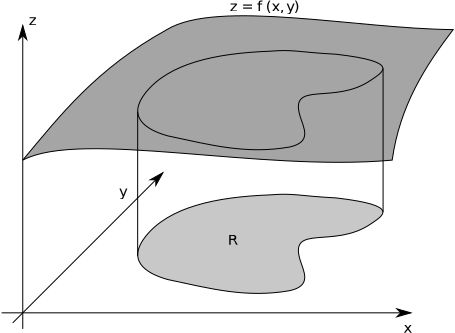
\includegraphics[width=0.6\textwidth]{doubleintegral3d.svg}
%%     \caption{Volume between region $R$ and surface $z$}
%%     \label{doubleintegral3d}
%%   \end{figure}
%% }{
%% \iftoggle{clearprint}{
%%   \begin{figure}[!htpb]
%%     \centering
%%     \def\svgwidth{0.7\columnwidth}
%%     \input{figures/latex/doubleintegral3d.pdf_tex}
%%     \caption{Volume between region $R$ and surface $z$}
%%     \label{doubleintegral3d}
%%   \end{figure}
%% }{
  \begin{figure}[H]
    \centering
    \def\svgwidth{0.6\columnwidth}
    \input{figures/latex/doubleintegral3d.pdf_tex}
    \caption{Volume between region $R$ and surface $z$}
    \label{doubleintegral3d}
  \end{figure}
%% }
%% }


  % Could put the technical, limit based definition here, or a note about how there is one.
  % It is somewhat hellish and definitely non-examinable.

  \subsubsection*{Properties of double integrals}

  Like single integrals, double integrals satisfy the usual linearity conditions:
    \begin{itemize}
      \item For a constant $c$,
    \[
      \iint_R cf(x, y) \, dA = c\iint_R f(x, y) \, dA;
    \]
      \item For functions $f(x, y)$ and $g(x, y)$,
    \[
      \iint_R f(x, y) + g(x, y) \, dA = \iint_R f(x, y)\, dA + \iint_R g(x, y) \, dA.
    \]
    \end{itemize}

  Also, if the region $R$ can be subdivided into regions $R_1$ and $R_2$ (figure (\ref{regionsubdivision})), then
    \[
      \iint_R f(x, y) \, dA = \iint_{R_1} f(x, y) \, dA + \iint_{R_2} f(x, y) \, dA.
    \]

%% \nextalt{Request description from lecturer or tactile diagram.}
%% \iftoggle{web}
%% {
%%   \begin{figure}[H]
%%     \centering
%%     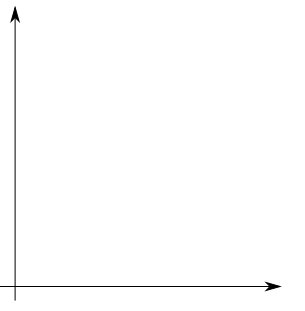
\includegraphics[width=0.4\textwidth]{regionsubdivision.svg}
%%     \caption{Region subdivision}
%%     \label{regionsubdivision}
%%   \end{figure}
%% }{
%% \iftoggle{clearprint}{
%%   \begin{figure}[!hbtp]
%%     \centering
%%     \def\svgwidth{0.4\columnwidth}
%%     \input{figures/latex/regionsubdivision.pdf_tex}
%%     \caption{Region subdivision}
%%     \label{regionsubdivision}
%%   \end{figure}
%% }{
  \begin{figure}[H]
    \centering
    \def\svgwidth{0.4\columnwidth}
    \input{figures/latex/regionsubdivision.pdf_tex}
    \caption{Region subdivision}
    \label{regionsubdivision}
  \end{figure}
%% }
%% }

  \subsubsection*{Evaluating double integrals with iterated integration}
	% Also changed "partial" to "iterated" in the title.  Which is more common?
	% The term "partial integration" does appear later as well.
	
	% I have rewritten the beginning of this section, with more justification.

  We will express the process of evaluating double integrals in terms of two single integrals: one with respect to $x$, one with respect to $y$.  We will start with the simplest possible regions (rectangles), then look at some more complicated ones.

  Suppose we want to evaluate the double integral of a function $f(x, y)$ over a rectangular region $R = [a, b] \times [c, d]$ (figure (\ref{rectangularregion2})).  
	
%% \nextalt{Request description from lecturer or tactile diagram.}
%% \iftoggle{web}
%% {
%%   \begin{figure}[H]
%%     \centering
%%     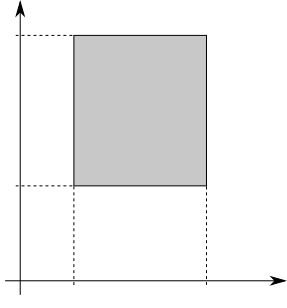
\includegraphics[width=0.45\textwidth]{rectangularregion2.svg}
%%     \caption{Rectangular region $R = [a, b] \times [c, d]$}
%%     \label{rectangularregion2}
%%   \end{figure}
%% }{
%% \iftoggle{clearprint}{
%%   \begin{figure}[!hbt]
%%     \centering
%%     \def\svgwidth{0.45\columnwidth}
%%     \input{figures/latex/rectangularregion2.pdf_tex}
%%     \caption{Rectangular region $R = [a, b] \times [c, d]$}
%%     \label{rectangularregion2}
%%   \end{figure}
%% }{
  \begin{figure}[H]
    \centering
    \def\svgwidth{0.45\columnwidth}
    \input{figures/latex/rectangularregion2.pdf_tex}
    \caption{Rectangular region $R = [a, b] \times [c, d]$}
    \label{rectangularregion2}
  \end{figure}
%% }
%% }
	
	Geometrically, this double integral is the volume $V$ of a solid. 	For a fixed value of $y$, the cross-sectional area of this solid is given by
    \[
      \int_a^b f(x, y) \, dx,
    \]
	by which we mean: integrate with respect to $x$, treat $y$ as a constant.  The result is a function of $y$.  Now suppose $y$ varies by a small increment $\Delta y$, giving a thin slice of the volume.  We can approximate the volume of the slice as
	  \[
		  \Delta V \approx \Delta y \int_a^b f(x, y) \, dx,
		\]
	the volume of a prism.  Thus
	  \[
		  \frac{\Delta V}{\Delta y} \approx \int_a^b f(x, y) \, dx.
		\]
	As $\Delta y \to 0$, this becomes an identity:
	  \[
		  \frac{dV}{dy} = \int_a^b f(x, y) \, dx.
		\]
	The volume from $y = c$ to $y = d$ is then
	  \[
		  \iint_R f(x, y) \, dA = \int_c^d \int_a^b f(x, y) \, dx \, dy.
		\]
		
	Notice that we could equally well have integrated with respect to $y$ first, to find the cross-sectional area for a fixed value of $x$, then integrated with respect to $x$ -- either order of integration would have given the volume of the solid, and therefore the same result.
	
	  \begin{theorem}[Fubini's Theorem -- special case]
    Let $R$ be the rectangle defined by
      \[
        a \leq x \leq b, \quad c \leq y \leq d.
      \]
    If $f(x, y)$ is continuous on $R$ then
    \[
      \iint_R f(x, y) \, dA = \int_c^d \int_a^b f(x, y) \, dx \, dy = \int_a^b \int_c^d f(x, y) \, dy \, dx.
    \]
  \end{theorem}

  \begin{example}
    Evaluate the double integral
      \[
        \iint_R 2xy \, dA
      \]
    where $R$ is the region defined by $1 \leq x \leq 3$, $2 \leq y \leq 4$.

    Using partial integration there are two possibilities: integrate first with respect to $x$, then $y$; or integrate first with respect to $y$, then $x$.  We will do both, then compare.
    \begin{align*}
      \int_2^4 \int_1^3 2xy \, dx \, dy & = \int_2^4 \left[ \int_1^3 2xy \, dx \right] dy  \\
      & = \int_2^4 \left[ x^2 y \right]_1^3 \, dy  \\
      & = \int_2^4 9y - y \, dy = \int_2^4 8y \, dy  \\
      & = \left[ 4y^2 \right]_2^4 = 4 \times 16 - 4 \times 4 = 48.
    \end{align*}
    \begin{align*}
      \int_1^3 \int_2^4 2xy \, dy \, dx & = \int_1^3 \left[ \int_2^4 2xy \, dy \right] dx  \\
      & = \int_1^3 \left[ xy^2 \right]_2^4 \, dx  \\
      & = \int_1^3 16x - 4x \, dx = \int_1^3 12x \, dx  \\
      & = \left[ 6x^2 \right]_1^3 = 6 \times 9 - 6 \times 1 = 48.
    \end{align*}
  So
  \[
    \int_2^4 \int_1^3 2xy \, dx \, dy = \int_1^3 \int_2^4 2xy \, dy \, dx.
  \]
  \end{example}
	

  \subsubsection*{Double integrals over non-rectangular domains}
	
	% There doesn't seem to be a sensible place to mention that this is using a more general version of Fubini's Theorem.

  In general this is very difficult, owing to the wide variety of possibilities for regions of the plane.  We'll look at certain types of non-rectangular regions that we can deal with.

  Consider a double integral
    \[
      \int_a^b \int_c^d f(x, y) \, dy \, dx.
    \]
  The inner partial integral (with respect to $y$) must give a function of $x$.  If $c$ and $d$ are functions of $x$, the resulting partial integral is still a function of $x$.  This allows us to integrate over regions of the form (figure (\ref{typeiregion})).
%% \nextalt{Request description from lecturer or tactile diagram.}
%% \iftoggle{web}
%% {
%%   \begin{figure}[H]
%%     \centering
%%     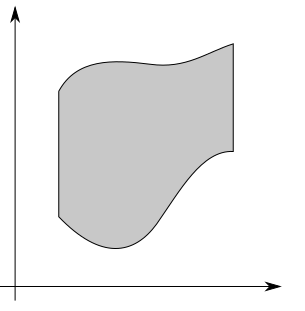
\includegraphics[width=0.4\textwidth]{typeiregion.svg}
%%     \caption{Type I region}
%%     \label{typeiregion}
%%   \end{figure}
%% }{
  \begin{figure}[H]
    \centering
    \def\svgwidth{0.4\columnwidth}
    \input{figures/latex/typeiregion.pdf_tex}
    \caption{Type I region}
    \label{typeiregion}
  \end{figure}
%% }

  The integral looks like
    \[
      \int_a^b \int_{g_1(x)}^{g_2(x)} f(x, y) \, dy \, dx.
    \]

  The outer limits must still be constant to give a numerical answer.

  Similarly, we can integrate over a region of the form (figure (\ref{typeiiregion}))
%% \nextalt{Request description from lecturer or tactile diagram.}
%% \iftoggle{web}
%% {
%%   \begin{figure}[H]
%%     \centering
%%     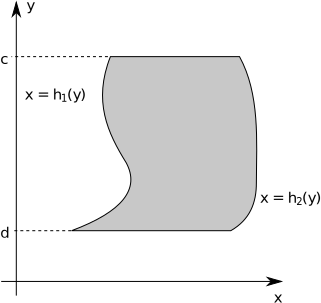
\includegraphics[width=0.47\textwidth]{typeiiregion.svg}
%%     \caption{Type II region}
%%     \label{typeiiregion}
%%   \end{figure}
%% }{
  \begin{figure}[H]
    \centering
    \def\svgwidth{0.47\columnwidth}
    \input{figures/latex/typeiiregion.pdf_tex}
    \caption{Type II region}
    \label{typeiiregion}
  \end{figure}
%% }
  using
    \[
      \int_c^d \int_{h_1(y)}^{h_2(y)} f(x, y) \, dx \, dy.
    \]

  % NOTE: I have cut two of these examples, one of which had a mistake, so save time since they took a whole lecture last year.
  \begin{examples}  
  \quad
    \begin{enumerate}
    \item Evaluate the integral
      \[
        \iint_R yx^2 \, dA,
      \]
    where $R$ is the region pictured in figure (\ref{regionexample1}).

%% \nextalt{Request description from lecturer or tactile diagram.}
%% \iftoggle{web}
%% {
%%   \begin{figure}[H]
%%     \centering
%%     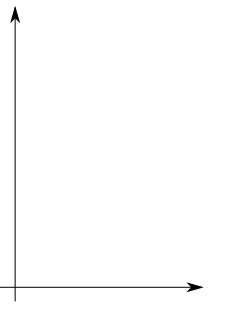
\includegraphics[width=0.35\textwidth]{regionexample1.svg}
%%     \caption{Example region 1}
%%     \label{regionexample1}
%%   \end{figure}
%% }{
  \begin{figure}[H]
    \centering
    \def\svgwidth{0.35\columnwidth}
    \input{figures/latex/regionexample1.pdf_tex}
    \caption{Example region 1}
    \label{regionexample1}
  \end{figure}
%% }

    \begin{align*}
      \int_0^1 \int_x^{2\sqrt{x}} yx^2 \, dy \, dx & = \int_0^1 \left[ \frac{y^2 x^2}{2} \right]_x^{2\sqrt{x}} \, dx = \int_0^1 x^3 - \frac{x^4}{2} \, dx  \\
      & = \left[ \frac{x^4}{4} - \frac{x^5}{10} \right]_0^1 = \frac{1}{4} - \frac{1}{10} = \frac{3}{20}.
    \end{align*}
    \item Some regions can be considered in either way -- especially those involving simple geometric shapes such as triangles.  In cases like this it may be that we can integrate in one order, but not the other.  In such situations, we may need to change the order of integration, as in the following integral.
    
    Calculate the double integral
      \[
        \int_0^2 \int_{x/2}^1 e^{y^2} \, dy \, dx.
      \]
    We cannot perform the $y$-integration first since we do not know an antiderivative of $e^{y^2}$.  Instead we will reverse the order of integration.  To find the new limits, we sketch the region of integration in figure (\ref{regionexample2}).
%% \nextalt{Request description from lecturer or tactile diagram.}
%% \iftoggle{web}
%% {
%%   \begin{figure}[H]
%%     \centering
%%     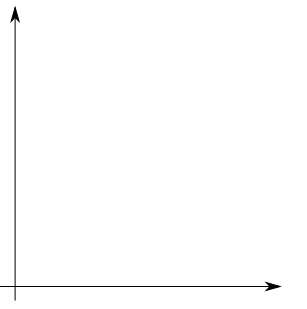
\includegraphics[width=0.4\textwidth]{regionexample4.svg}
%%     \caption{Example region 2}
%%     \label{regionexample2}
%%   \end{figure}
%% }{
  \begin{figure}[H]
    \centering
    \def\svgwidth{0.4\columnwidth}
    \input{figures/latex/regionexample4.pdf_tex}
    \caption{Example region 2}
    \label{regionexample2}
  \end{figure}
%% }

    In this region, $x$ varies from $0$ to the line $x = 2y$, and $y$ varies between $0$ and $1$.  Thus the integral is
      \begin{align*}
        \int_0^2 \int_{x/2}^1 e^{y^2} \, dy \, dx & = \int_0^1 \int_0^{2y} e^{y^2} \, dx \, dy  \\
        & = \int_0^1 \left[ xe^{y^2} \right]_0^{2y} \, dy  \\
        & = \int_0^1 2ye^{y^2} \, dy  \\
        & = \left[ e^{y^2} \right]_0^1 = e - 1.
      \end{align*}
    \end{enumerate}  
  \end{examples}



\subsection{Change of variable using the Jacobian}  \label{sect:Jacobian}

  Change of variable is the analogue of integration by substitution for double integrals.  It allows us to replace our variables $x$ and $y$ with new variables $u$ and $v$.  This can be useful for evaluating integrals over complicated regions.

  Suppose we want to evaluate the double integral of a function $f(x, y)$ over the region pictured in figure (\ref{regeval}).

%% \nextalt{Request description from lecturer or tactile diagram.}
%% \iftoggle{web}
%% {
%%  \begin{figure}[!htpb]
%%     \centering
%%     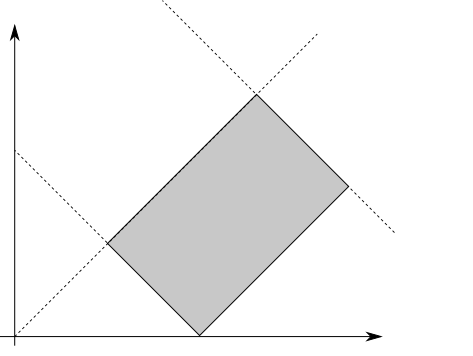
\includegraphics[width=0.6\textwidth]{JacobianRectanglexy.svg}
%%     \caption{Region of evaluation}
%%     \label{regeval}
%%   \end{figure}
%% }{
  \begin{figure}[!htpb]
    \centering
    \def\svgwidth{0.6\columnwidth}
    \input{figures/latex/JacobianRectanglexy.pdf_tex}
    \caption{Region of evaluation}
    \label{regeval}
  \end{figure}
%% }

  The region is rectangular, so integration ought to be easy -- but it's not because the sides of the rectangle are not parallel to the coordinate axes.  To evaluate this integral with the methods we already know we would need to divide the region into three subregions.
  % This is annoying/awkward.

  \emph{Solution:}  Draw some new axes!  We'll call them $u$ and $v$.  We want to choose them so that the region looks something like (figure (\ref{regnew})). 

%% \nextalt{Request description from lecturer or tactile diagram.}
%% \iftoggle{web}
%% {
%%   \begin{figure}[H]
%%     \centering
%%     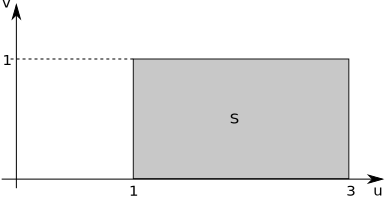
\includegraphics[width=0.6\textwidth]{JacobianRectangleuv.svg}
%%     \caption{Choose axes $u$ and $v$ to achieve this region}
%%     \label{regnew}
%%   \end{figure}
%% }{
  \begin{figure}[H]
    \centering
    \def\svgwidth{0.6\columnwidth}
    \input{figures/latex/JacobianRectangleuv.pdf_tex}
    \caption{Choose axes $u$ and $v$ to achieve this region}
    \label{regnew}
  \end{figure}
%% }

  How do we get from a point on the $(x, y)$-plane to the corresponding point on the $(u, v)$-plane?

  Define a \emph{transformation}
    \[
      U \colon \mathbb{R}^2 \longrightarrow \mathbb{R}^2
    \]
  where $U(x, y) = (u(x, y), v(x, y))$.

  To find $u$ and $v$ in terms of $x$ and $y$, we pick where we want our $u$- and $v$-axes to appear on the $(x, y)$-plane.

  $u$-axis: occurs when $v = 0$; should be parallel to the lines $y = x$ and $y = x - 1$, so pick
    \[
      v = x - y
    \]

  $v$-axis: occurs when $u = 0$; should be parallel to $y = 1 - x$ and $y = 3 - x$, so pick
    \[
      u = x + y
    \]

  So $U(x, y) = (x + y, x - y) = (u, v)$ takes a point on the $(x, y)$-plane, and gives a point on the $(u, v)$-plane.

  We want to use this to make a substitution that will turn
    \[
      \iint_R f(x, y) \, dA_{xy}
    \]
  (where $dA_{xy}$ is ``with respect to area on the $(x, y)$-plane'') into an integral in terms of $u$ and $v$, integrating over a region of the $(u, v)$-plane.

  \subsubsection*{Reminder: substitution for single integrals}

  If we have $x = g(u)$, then
    \[
      \int_a^b f(x) \, dx = \int_{g^{-1}(a)}^{g^{-1}(b)} f(g(u))g'(u) \, du.
    \]
  If $g$ is decreasing, $g'(u) < 0$, then $g^{-1}(b) < g^{-1}(a)$, so this is
    \begin{align*}
      \int_a^b f(x) \, dx & = - \int_{g^{-1}(b)}^{g^{-1}(a)} f(g(u))g'(u) \, du  \\
      & = \int_{g^{-1}(b)}^{g^{-1}(a)} f(g(u))\left|g'(u)\right| \, du.
    \end{align*}
  So in general,
    \[
      \int_a^b f(x) \, dx = \int_{\alpha}^{\beta} f(g(u))\left|g'(u)\right| \, du,
    \]
  where $\alpha$, $\beta$ are the $u$-limits, and $\alpha < \beta$.

  So we replace $dx$ with $\left|g'(u)\right|\, du$ (and swap the limits when $g'(u) < 0$).

  \subsubsection*{Change of variable for double integrals}

  For double integrals, we need to replace $dA_{x, y}$ (area on the $(x, y)$-plane) with something in terms of $dA_{uv}$ (area on the $(u, v)$-plane).  The expression we use is related to the derivatives of $x(u, v)$ and $y(u, v)$.

  \begin{definition}
    If $T \colon \mathbb{R}^2 \rightarrow \mathbb{R}^2$ is a transformation from the $(u, v)$-plane to the $(x, y)$-plane defined by
    \[
      x = x(u, v), \quad y - y(u, v),
    \]
    then the \emph{Jacobian of $T$}, denoted $\displaystyle{\frac{\partial(x, y)}{\partial(u, v)}}$ (or $J(u, v)$), is defined by
    \[
      \frac{\partial(x, y)}{\partial(u, v)} = \left|
      \begin{matrix}
        \dfrac{\strut\partial x}{\strut\partial u} & \dfrac{\strut\partial x}{\strut\partial v}  \\
        \dfrac{\strut\partial y}{\strut\partial u} & \dfrac{\strut\partial y}{\strut\partial v}
      \end{matrix}
      \right| = \frac{\partial x}{\partial u}\frac{\partial y}{\partial v} - \frac{\partial y}{\partial u}\frac{\partial x}{\partial v}.
    \]
  \end{definition}

  The Jacobian (named after 19th Century German mathematician Carl Jacobi) appears in place of $g'(u)$ in the change of variables formula.

  \begin{theorem}
    If the transformation $x = x(u, v)$, $y = y(u, v)$ maps the region $S$ in the $(u, v)$-plane to $R$ in the $(x, y)$-plane, and if $\displaystyle{\frac{\strut\partial(x, y)}{\strut\partial(u, v)}} \neq 0$ and does not change sign on $S$, then
      \[
        \iint_R f(x, y) \, dA_{xy} = \iint_S f(x(u, v), y(u, v)) \left|\displaystyle{\frac{\partial(x, y)}{\partial(u, v)}}\right| \, dA_{uv}.
      \]
  \end{theorem}

  \begin{example}
    We now use this to evaluate an integral over the rectangular region from the beginning of the section.  Consider
      \[
        \iint_R \frac{x - y}{x + y} \, dA_{xy},
      \]
    where $R$ is the rectangular region with vertices
      \[
        (1, 0), \quad \left(\frac{1}{2}, \frac{1}{2}\right), \quad \left(\frac{3}{2}, \frac{3}{2}\right), \quad (2, 1),
      \]
    as described at the beginning of the section.

    For our transformation from the $(x, y)$-plane to the $(u, v)$-plane, we chose
      \[
        u = x + y, \quad v = x - y.
      \]
    To find the Jacobian, we need to find $x$ and $y$ in terms of $u$ and $v$.
      \[
        u + v = x + y + x - y = 2x \implies x = \frac{u + v}{2},
      \]
      \[
        u - v = x + y - x + y = 2y \implies y = \frac{u - v}{2}.
      \]
    Hence
      \[
        \frac{\partial x}{\partial u} = \frac{1}{2}, \quad \frac{\partial x}{\partial v} = \frac{1}{2}, \quad \frac{\partial u}{\partial u} = \frac{1}{2}, \quad \frac{\partial y}{\partial v} = - \frac{1}{2},
      \]
    so the Jacobian is
      \[
        \left|
        \begin{matrix}
          \dfrac{\strut 1}{\strut 2} & \dfrac{\strut 1}{\strut 2}  \\
          \dfrac{\strut 1}{\strut 2} & - \dfrac{\strut 1}{\strut 2}
        \end{matrix}
        \right| = \frac{1}{2} \times \left(- \frac{1}{2}\right) - \frac{1}{2} \times \frac{1}{2} = - \frac{1}{4} - \frac{1}{4} = - \frac{1}{2}.
      \]
    So
      \begin{align*}
        \iint_R \frac{x - y}{x + y} \, dA_{xy} & = \iint_S \frac{v}{u} \times \left|- \frac{1}{2}\right| \, dA_{uv}  \\
        & = \int_0^1 \int_1^3 \frac{1}{2}\frac{v}{u} \, du \, dv  \\
        & = \frac{1}{2} \int_0^1 \left[v\ln\left|u\right|\right]_1^3 \, dv  \\
        & = \frac{1}{2}\ln(3)\int_0^1 v \, dv  \\
        & = \frac{1}{2}\ln(3)\left[\frac{1}{2}v^2\right]_0^1  \\
        & = \frac{1}{4}\ln(3).
      \end{align*}
  \end{example}

  Change of variable doesn't just work for rectangular regions -- with the right choice of variable, we can apply it to other regions as well, and even transform non-rectangular regions into rectangular ones.

  \begin{example}
    Evaluate
      \[
        \iint_R e^{xy} \, dA
      \]
    where $R$ is the region bounded by the lines
      \[
        y = \frac{1}{2}x, \quad y = x,
      \]
    and the hyperbolas
      \[
        y = \frac{1}{x}, \quad y = \frac{2}{x}.
      \]
 
%% \nextalt{Request description from lecturer or tactile diagram.}
%% \iftoggle{web}
%% {
%%   \begin{figure}[H]
%%     \centering
%%     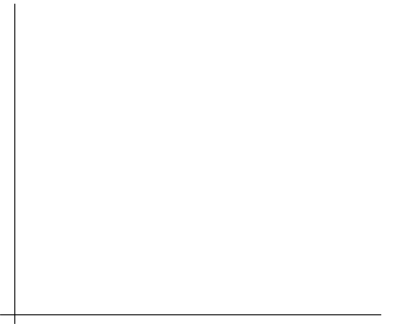
\includegraphics[width=0.6\textwidth]{JacobianHyperbolae.svg}
%%     \caption{Sketch of region}    
%%     \label{JacobianHyperbolae}
%%   \end{figure}
%% }{
  \begin{figure}[H]
    \centering
    \def\svgwidth{0.6\columnwidth}
    \input{figures/latex/JacobianHyperbolae.pdf_tex}
    \caption{Sketch of region}    
    \label{JacobianHyperbolae}
  \end{figure}
%% }

    We want a transformation that will change this region (figure (\ref{JacobianHyperbolae})) into a rectangle in the $(u, v)$-plane, so the boundary curves should correspond to constant values of $u$ and $v$.

    Rewrite the boundary curves as
      \[
        \frac{y}{x} = \frac{1}{2}, \quad \frac{y}{x} = 1, \quad xy = 1, \quad xy = 2.
      \]
    So try the transformation
      \[
        u = \frac{y}{x}, \quad v = xy.
      \]
    The lines in the $(u, v)$-plane corresponding to the boundary curves in the $(x, y)$-plane are
      \[
        u = \frac{1}{2}, \quad u = 1, \quad v = 1, \quad v = 2.
      \]
    This gives us our $u$-limits and $v$-limits.

    For the Jacobian, we need to express $x$ and $y$ in terms of $u$ and $v$:
      \[
        uv = \frac{y}{x} \times xy = y^2 \implies y = \sqrt{uv}
      \]
      \[
        \frac{v}{u} = xy \times \frac{x}{y} = x^2 \implies x = \sqrt{\frac{v}{u}}
      \]
    ($x$, $y$, $u$, $v$ are all positive on the region, so we can safely use the positive square roots)

    So the Jacobian is:
    \[
      \frac{\partial(x, y)}{\partial(u, v)} = \left|
      \begin{matrix}
        \dfrac{\strut\partial x}{\strut\partial u} & \dfrac{\strut\partial x}{\strut\partial v}  \\
        \dfrac{\strut\partial y}{\strut\partial u} & \dfrac{\strut\partial y}{\strut\partial v}
      \end{matrix}
      \right| =
      \left|
      \begin{matrix}
        - \dfrac{1}{2u}\sqrt{\dfrac{v}{u}} & \dfrac{1}{2\sqrt{uv}}  \\
        \dfrac{1}{2}\sqrt{\dfrac{v}{u}} & \dfrac{1}{2}\sqrt{\dfrac{u}{v}}
      \end{matrix}
      \right| = - \frac{1}{4u} - \frac{1}{4u} = - \frac{1}{2u}.
    \]
    Observe that, unlike in the previous example, this Jacobian is not constant.

     Thus the integral is
       \begin{align*}
         \iint_R e^{xy} \, dA_{xy} & = \iint_S e^v \left|-\frac{1}{2u}\right| \, dA_{uv}  \\
         & = \frac{1}{2} \iint_S \frac{1}{u}e^v \, dA_{uv}  \\
         & = \frac{1}{2} \int_1^2 \int_{1/2}^1 \frac{1}{u}e^v \, du \, dv  \\
         & = \frac{1}{2} \int_1^2 \left[e^v\ln\left|u\right|\right]_{1/2}^1 \, dv  \\
         & = \frac{1}{2}\ln(2)\int_1^2 e^v \, dv  \\
         & = \frac{1}{2}(e^2 - e)\ln(2).
       \end{align*}
  \end{example}



\subsection{Polar coordinates}

  In Section~\ref{sect:Jacobian} we saw that, for integrals over certain awkward-shaped regions, it is convenient to be able to transform the plane to a new set of coordinate axes.

  In the examples we've seen so far this transformation gave us a new cartesian plane.  In this section we look at a different coordinate system: \emph{polar coordinates}.

  \subsubsection*{Cartesian coordinates:}

  \begin{itemize}
    \item Two perpendicular axes (figure (\ref{cartesian})).
    \item Specify a point on the plane using two real numbers, $x$ and $y$ -- horizontal and vertical distances from origin.
    \item Each point $P$ has unique $(x, y)$-coordinates.
    \item Named after Ren\'e Descartes.  Also known as rectangular coordinates.
  \end{itemize}

%% \nextalt{Request description from lecturer or tactile diagram.}
%% \iftoggle{web}
%% {
%%   \begin{figure}[H]
%%     \centering
%%     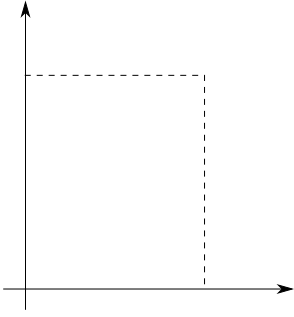
\includegraphics[width=0.3\textwidth]{cartesian.svg}
%%     \caption{Cartesian coordinates}
%%     \label{cartesian}
%%   \end{figure}
%% }{
  \begin{figure}[H]
    \centering
    \def\svgwidth{0.3\columnwidth}
    \input{figures/latex/cartesian.pdf_tex}
    \caption{Cartesian coordinates}
    \label{cartesian}
  \end{figure}
%% }


  \subsubsection*{Polar coordinates:}

%% \nextalt{Request description from lecturer or tactile diagram.}
%% \iftoggle{web}
%% {
%%   \begin{figure}[H]
%%     \centering
%%     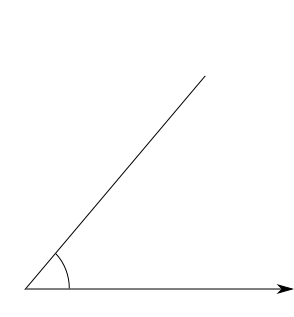
\includegraphics[width=0.29\textwidth]{polar.svg}
%%     \caption{Polar coordinates}
%%     \label{polar}
%%   \end{figure}
%% }{
  \begin{figure}[H]
    \centering
    \def\svgwidth{0.29\columnwidth}
    \input{figures/latex/polar.pdf_tex}
    \caption{Polar coordinates}
    \label{polar}
  \end{figure}
%% }

  \begin{itemize}
    \item One axis (``polar axis'') -- like positive half of the cartesian $x$-axis, with origin $O$ (figure (\ref{polar})).
    \item Specify a point $P$ by two real numbers:
      \begin{itemize}
        \item $r$ (``radius''): distance from the origin;
        \item $\theta$ : anticlockwise angle between axis and line segment from $O$ to $P$.
      \end{itemize}
    \item For a given $P$, $r$ is unique, but $\theta$ is not, since:
      \[
        (r, \theta) = (r, \theta + 2k\pi), \quad k \in \mathbb{Z}.
      \]
    \item $(0, \theta)$ is the origin for all values of $\theta$.
  \end{itemize}

  \subsubsection*{Relationship between polar and cartesian coordinates}

  We can move between polar and cartesian coordinates.  Consider figure (\ref{polarcartesian}).
%% \nextalt{Request description from lecturer or tactile diagram.}
%% \iftoggle{web}
%% {
%%   \begin{figure}[H]
%%     \centering
%%     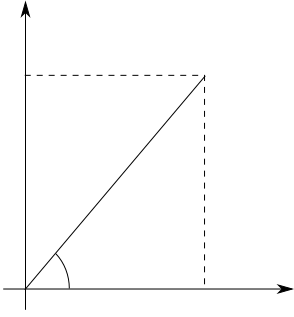
\includegraphics[width=0.29\textwidth]{polarcartesian.svg}
%%     \caption{Triangle with vertices $(0, 0)$, $(x, 0)$, $(x, y)$}
%%     \label{polarcartesian}
%%   \end{figure}
%% }{
  \begin{figure}[H]
    \centering
    \def\svgwidth{0.29\columnwidth}
    \input{figures/latex/polarcartesian.pdf_tex}
    \caption{Triangle with vertices $(0, 0)$, $(x, 0)$, $(x, y)$}
    \label{polarcartesian}
  \end{figure}
%% }

  Considering the triangle with vertices $(0, 0)$, $(x, 0)$, $(x, y)$, we observe that
    \[
      \cos(\theta) = \frac{x}{r}, \quad \sin(\theta) = \frac{y}{r},
    \]
  so to change from polar to cartesian coordinates, use the transformation
    \[
      x = r\cos(\theta), \quad y = r\sin(\theta).
    \]

  Changing from cartesian to polar coordinates is a bit trickier.  By Pythagoras' Theorem:
    \[
      r^2 = x^2 + y^2.
    \]
  There is no easy formula for $\theta$, but we can use
    \[
      \tan(\theta) = \frac{y}{x}.
    \]
  Note that $\arctan$ gives values between $-\dfrac{\pi}{2}$ and $\dfrac{\pi}{2}$, so $\arctan$ will not consistently give the value of $\theta$.

  \subsubsection*{Equations of curves in polar coordinates}
  % NOTE: I'm leaving this in the notes for now, though I may cut it from the lectures if I am running low on time -- which is likely given last year's timings.

  Some curves are much easier to write in polar coordinates than in cartesian coordinates.

  \begin{examples}
    \begin{enumerate}
      \item Circle of radius $a$.
        
        In cartesian coordinates:
          \[
            x^2 + y^2 = a^2,
          \]
        or
          \[
            y = \sqrt{a^2 - x^2}, \quad y = - \sqrt{a^2 - x^2}.
          \]
        In polar coordinates:
          \[
            r = a.
          \]
        This will be very useful for simplifying integrals over circular regions.
      \item Spirals: Archimedean spiral (figure (\ref{arch})), $r = a\theta$, $a$ constant and Logarithmic spiral (figure (\ref{log})), $r = ae^{b\theta}$, $a$, $b$ constant.

        %% \nextalt{Request description from lecturer or tactile diagram.}
        \begin{figure}[!htbp]
          \centering
          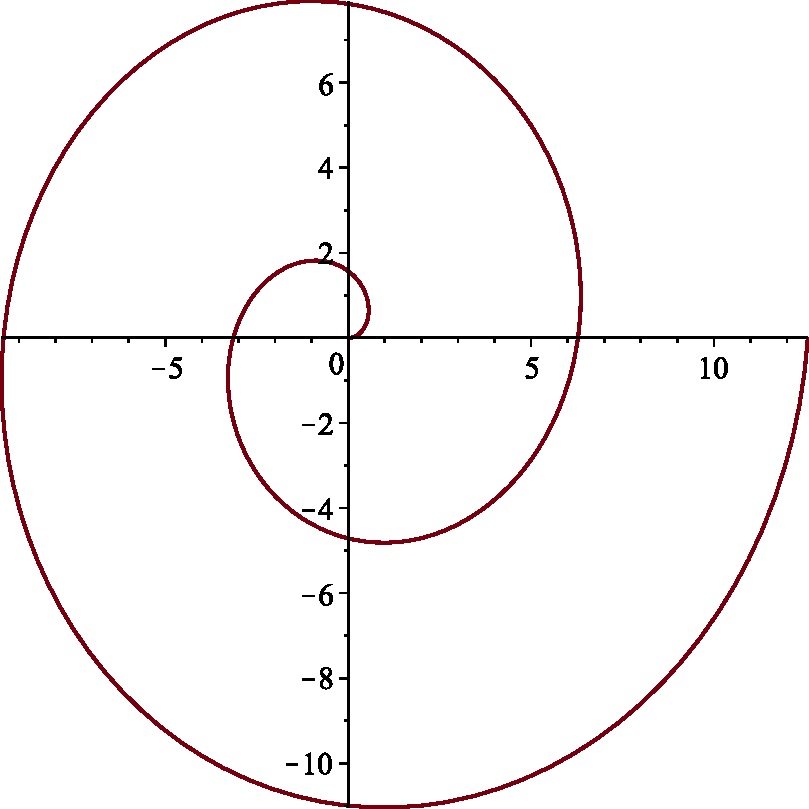
\includegraphics[width=0.5\textwidth]{archspiral.pdf}
          \caption{Archimedean spiral}
          \label{arch}
        \end{figure}

        %% \nextalt{Request description from lecturer or tactile diagram.}
        \begin{figure}[!hbtp]
          \centering
          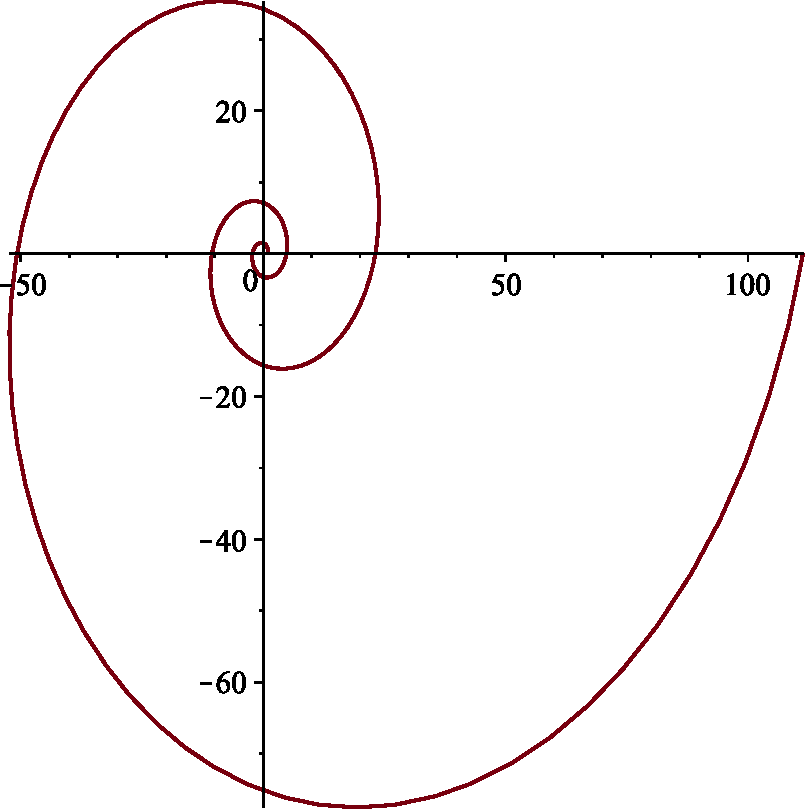
\includegraphics[width=0.5\textwidth]{logspiral.pdf}
          \caption{Logarithmic spiral}
          \label{log}
        \end{figure}
        
      \item Cardioids (figure (\ref{card})): $r = a \pm a\sin(\theta)$ and $a \pm a\cos(\theta)$, $a$ constant.

        %% \nextalt{Request description from lecturer or tactile diagram.}
        \begin{figure}[!htpb]
          \centering
          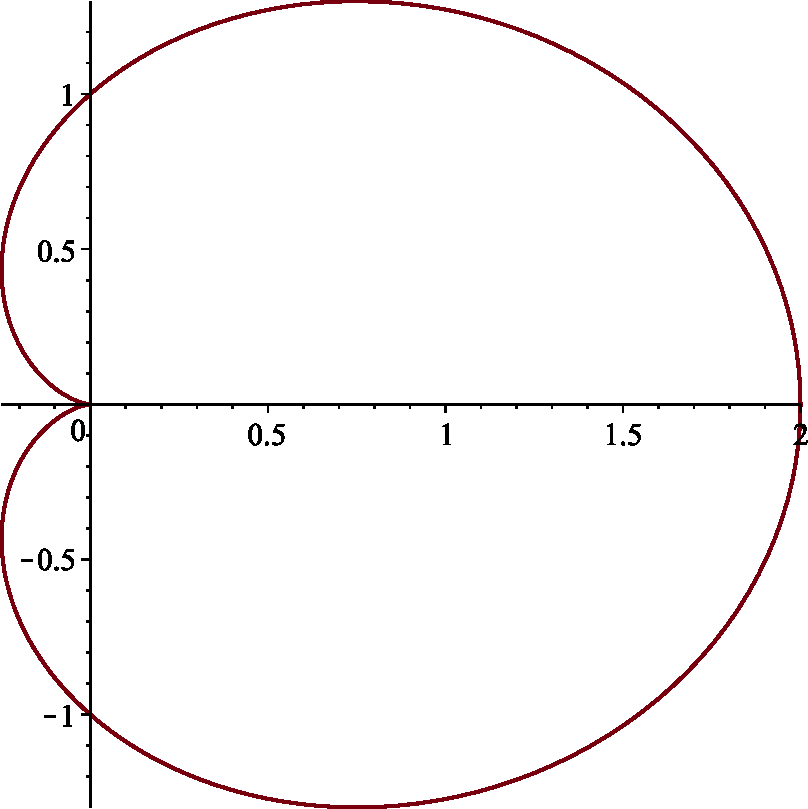
\includegraphics[width=0.5\textwidth]{cardioid.pdf}
          \caption{Cardioid}
          \label{card}
        \end{figure}

        More generally: lima\c{c}ons $r = a \pm b\sin(\theta)$, $r = a \pm b\cos(\theta)$, $a$, $b$ constants.
    \end{enumerate}
  \end{examples}
  
  \subsubsection*{Simple polar regions}
  
  When we use polar coordinates for integration, we will integrate over a particular kind of region that is straightforward to express in polar coordinates, called a \emph{simple polar region}.
  
  \begin{definition}
    A \emph{simple polar region} is a region of the plane enclosed between two \emph{rays} $\theta = \alpha$, $\theta = \beta$, and two (continuous) curves $r = r_1(\theta)$, $r = r_2(\theta)$, satisfying
    \[
      \alpha \leq \beta, \quad \beta - \alpha \leq 2\pi, \quad 0 \leq r_1(\theta) \leq r_2(\theta).
    \]
  \end{definition}
  
  An example is shown in the diagram (\ref{simplepolarregion}).
  
%% \nextalt{Request description from lecturer or tactile diagram.}
%% \iftoggle{web}
%% {
%%   \begin{figure}[H]
%%     \centering
%%     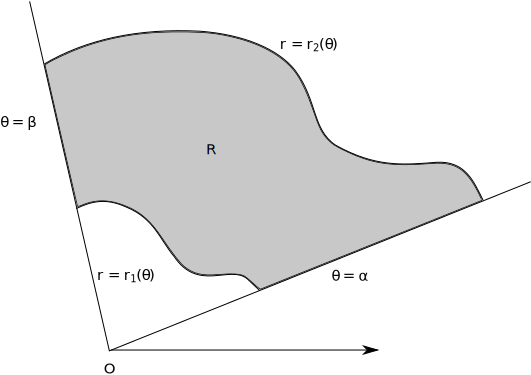
\includegraphics[width=0.7\textwidth]{simplepolarregion.svg}
%%     \caption{A simple polar region}
%%     \label{simplepolarregion}
%%   \end{figure}
%% }{
  \begin{figure}[H]
    \centering
    \def\svgwidth{0.7\columnwidth}
    \input{figures/latex/simplepolarregion.pdf_tex}
    \caption{A simple polar region}
    \label{simplepolarregion}
  \end{figure}
%% }


\subsection{Double integrals in polar coordinates}

  Using change of variable and the Jacobian, we can convert an integral in cartesian coordinates into an integral in polar coordinates.  This can simplify certain integrals, especially those over circular regions, and those involving $x^2 + y^2$.

  \begin{example}[Volume of a sphere]
    In cartesian coordinates, a sphere of radius $a$ has the equation
      \[
        x^2 + y^2 + z^2 = a^2,
      \]
    or:
      \[
        \text{upper hemisphere: } z = \sqrt{a^2 - x^2 - y^2},
      \]
      \[
        \text{lower hemisphere: } z = - \sqrt{a^2 - x^2 - y^2}.
      \]
    So the volume of the sphere is
      \[
        V = 2\iint_R \sqrt{a^2 - x^2 - y^2} \, dA,
      \]
    where $R$ is the circular region bounded by
      \[
        x^2 + y^2 = a^2.
      \]
    Thus in cartesian coordinates, the integral is:
      \[
        V = 2\int\nolimits_{-a}^a \int\nolimits_{-\sqrt{a^2 - x^2}}^{\sqrt{a^2 - x^2}} \sqrt{a^2 - x^2 - y^2} \, dy \, dx.
      \]
    This is complicated.  We can simplify it by changing to polar coordinates.  We have
      \[
        x = r\cos(\theta), \quad y = r\sin(\theta),
      \]
    so the Jacobian is
    \[
      \frac{\partial(x, y)}{\partial(r, \theta)} = \left|
      \begin{matrix}
        \dfrac{\strut\partial x}{\strut\partial r} & \dfrac{\strut\partial x}{\strut\partial \theta}  \\
        \dfrac{\strut\partial y}{\strut\partial r} & \dfrac{\strut\partial y}{\strut\partial \theta}
      \end{matrix}
      \right| =
      \left|
      \begin{matrix}
        \cos(\theta) & -r\sin(\theta)  \\
        \sin(\theta) & r\cos(\theta)
      \end{matrix}
      \right| = r\cos^2(\theta) + r\sin^2(\theta) = r.
    \]
    Note that the region $R$ is a simple polar region; the boundary rays and curves give the following limits for the integral:
      \[
        0 \leq \theta \leq 2\pi,
      \]    
      \[
        0 \leq r \leq a.
      \]
    Thus the volume is
      \begin{align*}
        V & = 2\int_0^{2\pi} \int_0^a r\sqrt{a^2 - r^2} \, dr \, d\theta  \\
        & = \int_0^{2\pi} \left[-\frac{2}{3} (a^2 - r^2)^{3/2}\right]_0^a \, d\theta  \\
        & = \int_0^{2\pi} \left(-\frac{2}{3}(a^2 - a^2)^{3/2} + \frac{2}{3}(a^2 - 0^2)^{3/2}\right) \, d\theta  \\
        & = \int_0^{2\pi} \frac{2}{3}a^3 d\theta  \\
        & = \left[\frac{2}{3}a^3\theta\right]_0^{2\pi}  \\
        & = \frac{4}{3}\pi a^3.
      \end{align*}
    This agrees with the standard formula for the volume of a sphere.
  \end{example}

  In this example we started with the integrand and limits in cartesian coordinates, and converted to polar coordinates, using the Jacobian to change variable.  However, we may be given the integrand and limits in polar form originally.  In this case, although we don't need to make a change of variable, we still need to multiply the integrand by the Jacobian.

  \begin{theorem}
    If $R$ is a simple polar region bounded by the rays $\theta = \alpha$, $\theta = \beta$, and the curves $r = r_1(\theta)$, $r = r_2(\theta)$, and if $f(r, \theta)$ is continuous on $R$, then
      \[
        \iint_R f(r,\theta) \, dA = \int_{\alpha}^{\beta} \int_{r_1(\theta)}^{r_2(\theta)} f(r, \theta) r \, dr \, d\theta.
      \]
  \end{theorem}

  We won't prove this theorem, but here is an explanation of why it is true:

  Double integration treats regions with constant limits as rectangles, but in polar coordinates such regions are not rectangular.  Consider, for example figure (\ref{notrectangles}).
  
%% \nextalt{Request description from lecturer or tactile diagram.}
%% \iftoggle{web}
%% {
%%   \begin{figure}[H]
%%     \centering
%%     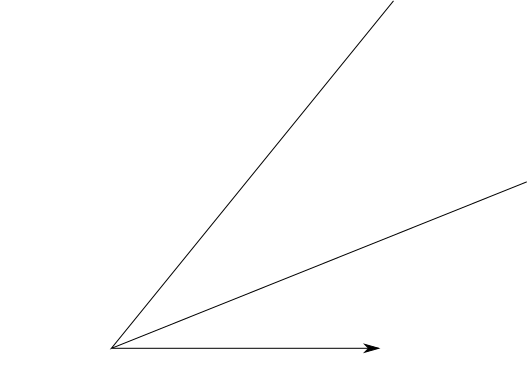
\includegraphics[width=0.55\textwidth]{notrectangles.svg}
%%     \caption{Region which is not rectangular}
%%     \label{notrectangles}
%%   \end{figure}
%% }{
  \begin{figure}[H]
    \centering
    \def\svgwidth{0.55\columnwidth}
    \input{figures/latex/notrectangles.pdf_tex}
    \caption{Region which is not rectangular}
    \label{notrectangles}
  \end{figure}
%% }
  
  Double integration treats the regions $R_1$ and $R_2$ as rectangles with the same area -- but they're not rectangles, and $R_2$ is much larger than $R_1$.  The contribution made to the area of a region is proportional to the distance from the origin (i.e. proportional to the radius).  This explains why the Jacobian is $r$.
  
  When we use double integration to integrate something in polar form, we are effectively changing variable to a cartesian $(r, \theta)$-plane.  Note that $r$ is always positive, and $\theta$ is between $0$ and $2\pi$, but that otherwise this is a standard cartesian plane and that regions with constant limits are now rectangular.

  \begin{example}
    Evaluate the double integral
      \[
        \iint_R \sin(\theta) \, dA,
      \]
    where $R$ is the region in the first quadrant between the the circle $r = 2$ and the cardioid $r = 2 + 2\cos(\theta)$ (figure (\ref{cardioidcircle})).
    
%% \nextalt{Request description from lecturer or tactile diagram.}
%% \iftoggle{web}
%% {
%%   \begin{figure}[H]
%%     \centering
%%     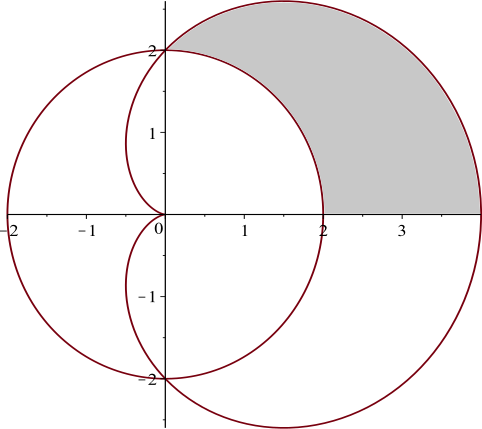
\includegraphics[width=0.5\textwidth]{cardioidcircle.svg}
%%     \caption{Region $R$}
%%     \label{cardioidcircle}
%%   \end{figure}
%% }{  
  \begin{figure}[H]
    \centering
    \def\svgwidth{0.5\columnwidth}
    \input{figures/latex/cardioidcircle.pdf_tex}
    \caption{Region $R$}
    \label{cardioidcircle}
  \end{figure}
%% }
  
    Observe that $R$ is a simple polar region, with limits given by
      \[
        0 \leq \theta \leq \frac{\pi}{2},
      \]
      \[
        2 \leq r \leq 2 + 2\cos(\theta).
      \]
    Thus the integral is
      \begin{align*}
        \iint_R \sin(\theta) \, dA & = \int\nolimits_0^{\pi/2} \int\nolimits_2^{2 + 2\cos(\theta)} \sin(\theta)r \, dr \, d\theta  \\
        & = \int_0^{\pi/2} \left[\frac{1}{2}r^2\sin(\theta)\right]_2^{2 + 2\cos(\theta)} \, d\theta  \\
        & = 2\int_0^{\pi/2} (1 + \cos(\theta))^2 \sin(\theta) - \sin(\theta) \, d\theta  \\
        & = 2\left[-\frac{1}{3}(1 + \cos(\theta))^3 + \cos(\theta)\right]_0^{\pi/2}  \\
        & = 2\left(-\frac{1}{3}-\left(-\frac{5}{3}\right)\right)  \\
        & = \frac{8}{3}.
      \end{align*}
  \end{example}
  
  
  
\subsection{Triple integrals}

  As with partial differentiation, we can extend double integration to higher numbers of variables.  We will look at integration in the $3$ variable case (we won't go any higher than this).

  \subsubsection*{$3$-dimensional regions}

  \emph{Double integrals:} integrate over a $2$D region of the $(x, y)$-plane.

  \emph{Triple integrals:} integrate over a $3$D region of $(x, y, z)$-space.

  For us, this will always be a finite solid.

  \emph{Notation}

  The triple integral of a function of $3$ variables, $f(x, y, z)$, over a $3$-dimensional region $G$ is denoted
    \[
      \iiint_G f(x, y, z) \, dV.
    \]
  You should read $dV$ as ``with respect to volume''.  The $G$ doesn't stand for anything -- unlike the case of double-integrals (where we use $R$) there is no standard letter used for $3$D regions.
  % I have followed Anton et al.

  \subsubsection*{What does it respresent?}

  In the $1$ and $2$ variable cases, definite integrals represented a tangible geometric quantity.

  \emph{Single integrals:} area under a curve.

  \emph{Double integrals:} volume under a surface.

  \emph{Triple integrals:} ?

  We live in a universe with $3$ spacial dimensions, but a triple integral is something $4$-dimensional, so we don't have the words to describe what it represents geometrically.

  Triple integrals can tell us about physical quantities though.  For example:
    \begin{itemize}
      \item mass of an object (integrate its density)
      \item centre of mass/centre of gravity
      \item volume
      \item gravitational potential
      \item magnetic and electric fields
      \item position of a particle in quantum physics
    \end{itemize}

  \subsubsection*{Properties of triple integrals}

  As with single and double integrals, we have the usual linearity properties:
    \begin{itemize}
      \item For a constant $c$,
    \[
      \iiint_G cf(x, y, z) \, dV = c\iiint_G f(x, y, z) \, dV;
    \]
      \item For functions $f(x, y, z)$ and $g(x, y, z)$,
    \[
      \iiint_G f(x, y, z) + g(x, y, z) \, dV = \iiint_G f(x, y, z)\, dV + \iiint_G g(x, y, z) \, dV.
    \]
    \end{itemize}

  Also, if the region $G$ can be subdivided into regions $G_1$ and $G_2$, then
    \[
      \iiint_G f(x, y, z) \, dV = \iiint_{G_1} f(x, y, z) \, dV + \iiint_{G_2} f(x, y, z) \, dV.
    \]

  \subsubsection*{Triple integrals over cuboids}

  For double integrals, the simplest regions for integration were rectangular boxes.

  Similarly, for triple integration, the simplest regions are cuboids -- like the case of evaluating double integrals over rectangles, triple integrals over cuboids have constant limits.

  \begin{theorem}
    Let $G$ be the cuboid defined by
      \[
        a \leq x \leq b, \quad c \leq y \leq d, \quad k \leq z \leq l.
      \]
    If $f(x, y, z)$ is continuous on the region $G$, then
      \[
        \iiint_G f(x, y, z) \, dV = \int_a^b \int_c^d \int_k^l f(x, y, z) \, dz \, dy \, dx.
      \]
    Moreover, in the integral on the right, one can alter the order of integration, without changing the resulting value of the integral.
  \end{theorem}

  For triple integrals, there are six possible orders of integration.  In the following example we will evaluate a triple integral using one of these orders, but any other order would give the same result.

  \begin{example}
    Evaluate the triple integral
      \[
        \iiint_G 6x^3y^2z \, dV
      \]
    over the cuboid $G$ defined by
      \[
        1 \leq x \leq 2, \quad -1 \leq y \leq 1, \quad 0 \leq z \leq 2.
      \]

      \begin{align*}
        \iiint_G 6x^3y^2z \, dV & = \int_1^2 \int_{-1}^1 \int_0^2 6x^3y^2z \, dz \, dy \, dx  \\
        & = \int_1^2 \int_{-1}^1 \left[3x^3y^2z^2\right]_0^2 \, dy \, dx  \\
        & = \int_1^2 \int_{-1}^1 12x^3y^2 \, dy \, dx  \\
        & = \int_1^2 \left[4x^3y^3\right]_{-1}^1 \, dx  \\
        & = \int_1^2 8x^3 \, dx  \\
        & = \left[2x^4\right]_1^2 = 2 \times 16 - 2 = 30.
      \end{align*}
  \end{example}

  \subsubsection*{More general regions}

  In the $2$-variable case we looked at regions of the form in figure (\ref{typeiregion2}).
%% \nextalt{Request description from lecturer or tactile diagram.}
%% \iftoggle{web}
%% {
%%   \begin{figure}[H]
%%     \centering
%%     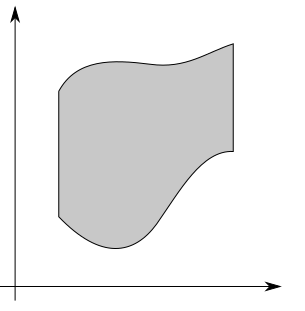
\includegraphics[width=0.45\textwidth]{typeiregion.svg}
%%     \caption{Type I region}
%%     \label{typeiregion2}
%%   \end{figure}
%% }{
  \begin{figure}[H]
    \centering
    \def\svgwidth{0.45\columnwidth}
    \input{figures/latex/typeiregion.pdf_tex}
    \caption{Type I region}
    \label{typeiregion2}
  \end{figure}
%% }

  In the $3$-variable case, we generalise this by replacing
    \begin{itemize}
      \item $[a, b]$ with a region $R$ of the $(x, y)$-plane (one we can perform double integration over);
      \item the curves $y = g_1(x)$ and $y=g_2(x)$ with surfaces $z = g_1(x, y)$ and $z = g_2(x, y)$.
    \end{itemize}

  This gives regions $G$ of the form shown in figure (\ref{tripleform}).
%% \nextalt{Request description from lecturer or 3D object.}
%% \iftoggle{web}
%% {
%%   \begin{figure}[!htbp]
%%     \centering
%%     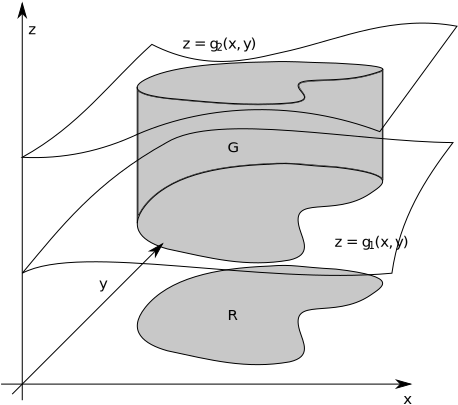
\includegraphics[width=0.63\textwidth]{tripleintegral3dregion.svg}
%%     \caption{Form of regions}
%%     \label{tripleform}
%%   \end{figure}
%% }{
  \begin{figure}[!htbp]
    \centering
    \def\svgwidth{0.63\columnwidth}
    \input{figures/latex/tripleintegral3dregion.pdf_tex}
    \caption{Form of regions}
    \label{tripleform}
  \end{figure}
%% }

  \emph{Terminology:}
    \begin{itemize}[topsep=0pt]
      \item $G$ is called a \emph{simple $xy$-solid};
      \item $z = g_1(x, y)$ is the \emph{lower surface};
      \item $z = g_2(x, y)$ is the \emph{upper surface}.
    \end{itemize}

  \begin{theorem}
    For a simple $xy$-solid $G$, as described above, and $f(x, y, z)$ continuous on $G$,
      \[
        \iiint_G f(x, y, z) \, dV = \iint_R \left[\int_{g_1(x, y)}^{g_2(x, y)} f(x, y, z) \, dz \right] \, dA.
      \]
  \end{theorem}

  \begin{example}
    Evaluate the triple integral
      \[
        \iiint_G z \, dV.
      \]
    where $G$ is the simple $xy$-solid bounded by
      \[
        g_1(x, y) = -\sqrt{1 - y^2}, \quad g_2(x, y) = \sqrt{1 - y^2},
      \]
    and the projection of $G$ onto the $(x, y)$-plane is the triangle (figure (\ref{tripleregionxyplane})) with vertices
      \[
        (0, 0), \quad (0, 1), \quad (1, 1).
      \]
%% \nextalt{Request description from lecturer or tactile diagram.}
%% \iftoggle{web}
%% {
%%   \begin{figure}[H]
%%     \centering
%%     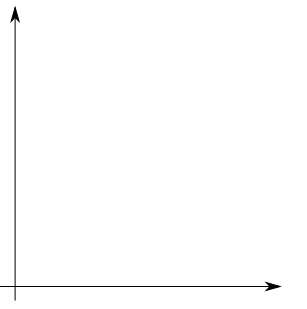
\includegraphics[width=0.32\textwidth]{tripleregionxyplane.svg}
%%     \caption{Projection of $G$ onto the $(x,y)$-plane}
%%     \label{tripleregionxyplane}
%%   \end{figure}
%% }{
  \begin{figure}[H]
    \centering
    \def\svgwidth{0.32\columnwidth}
    \input{figures/latex/tripleregionxyplane.pdf_tex}
    \caption{Projection of $G$ onto the $(x,y)$-plane}
    \label{tripleregionxyplane}
  \end{figure}
%% }

    From the diagram, we have
      \begin{itemize}[topsep=0pt]
        \item $y$-limits: $x$ and $1$;
        \item $x$-limits: $0$ and $1$.
      \end{itemize}
    Thus the integral is
      \begin{align*}
        \iiint_G z \, dV & = \int_0^1 \int_x^1 \int_{-\sqrt{1 - y^2}}^{\sqrt{1 - y^2}} z \, dz \, dy \, dx  \\
        & = \int_0^1 \int_x^1 \left[\frac{1}{2}z\right]_{-\sqrt{1 - y^2}}^{\sqrt{1 - y^2}} \, dy \, dx  \\
        & = \int_0^1 \int_x^1 1 - y^2 \, dy \, dx  \\
        & = \int_0^1 \left[y - \frac{y^3}{3}\right]_x^1 \, dx  \\
        & = \int_0^1 1 - \frac{1}{3} - x + \frac{x^3}{3} \, dx  \\
        & = \int_0^1 \frac{x^3}{3} - x + \frac{2}{3} \, dx  \\
        & = \left[\frac{x^4}{12} - \frac{x^2}{2} + \frac{2}{3}x\right]_0^1  \\
        & = \frac{1}{12} - \frac{1}{2} + \frac{2}{3}  \\
        & = \frac{1}{4}.
      \end{align*}
  \end{example}  




\subsection{Triple integrals in spherical coordinates}
  
  % ``a lot'' too colloquial?
  % This was written in 30 seconds and needs rewording.  I will not write it out in the lecture anyway.
  There are a lot of possibilities for three-dimensional regions, and so far we can only integrate over a very narrow range of possibilities.  In order to expand our possibilities for regions to integrate over, we will use an alternative coordinate system called \emph{spherical coordinates}.

  Spherical coordinates are a $3$-dimensional analogue of polar coordinates (figure (\ref{spherical})).  In this case we have three coordinates:
    \begin{itemize}
      \item radius $r$ (sometimes denoted $\rho$), the distance from the origin;
      \item $\theta$, the angle from the positive $x$-axis (called the \emph{azimuthal} angle);
      \item $\varphi$, the angle from the positive $z$-axis (called the \emph{polar} angle).
    \end{itemize}
  
%% \nextalt{Request description from lecturer or 3D object.}
%% \iftoggle{web}
%% {
%%   \begin{figure}[H]
%%     \centering
%%     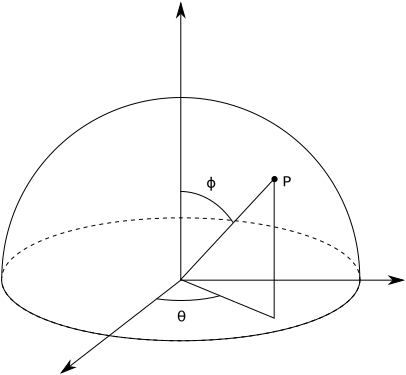
\includegraphics[width=0.5\textwidth]{spherical.svg}
%%     \caption{Spherical coordinates}
%%     \label{spherical}
%%   \end{figure}
%% }{
  \begin{figure}[H]
    \centering
    \def\svgwidth{0.5\columnwidth}
    \input{figures/latex/spherical.pdf_tex}
    \caption{Spherical coordinates}
    \label{spherical}
  \end{figure}
%% }
    
  \subsubsection*{Converting between spherical and cartesian coordinates}
  
  As in the two dimensional case with polar coordinates, we can convert between the spherical and cartesian coordinate systems.
  
  To convert from spherical to cartesian coordinates, use:
    \begin{align*}
      x & = r\sin(\varphi)\cos(\theta),  \\
      y & = r\sin(\varphi)\sin(\theta),  \\
      z & = r\cos(\varphi).
    \end{align*}
  As for polar coordinates, these can all be derived geometrically by considering the appropriate right-angled triangles.
  
  To convert from cartesian to spherical coordinates, use:
    \begin{align*}
      r & = \sqrt{x^2 + y^2 + z^2},  \\
      \tan(\theta) & = \frac{y}{x},  \\
      \cos(\varphi) & = \frac{z}{\sqrt{x^2 + y^2 + z^2}}.
    \end{align*}
  
  
  
%\subsection{Triple integrals in spherical coordinates}
  
  As in the case of polar coordinates, evaluating a triple integral uses the Jacobian for the transformation from spherical to cartesian coordinates.  We haven't covered change of variable for triple integrals, but it proceeds in the same way as for double integrals.  The Jacobian looks like
  \[
    \frac{\partial(x, y, z)}{\partial(r, \theta, \varphi)} = \left|
      \begin{matrix}
        \dfrac{\strut\partial x}{\strut\partial r} & \dfrac{\strut\partial x}{\strut\partial \theta} & \dfrac{\strut\partial x}{\strut\partial \varphi}  \\
        \dfrac{\strut\partial y}{\strut\partial r} & \dfrac{\strut\partial y}{\strut\partial \theta} & \dfrac{\strut\partial y}{\strut\partial \varphi}  \\
        \dfrac{\strut\partial z}{\strut\partial r} & \dfrac{\strut\partial z}{\strut\partial \theta} & \dfrac{\strut\partial z}{\strut\partial \varphi}
      \end{matrix}
      \right|
  \]
  
  This is the determinant of a $3 \times 3$ matrix.  We won't go into details of how to calculate these (for anyone interested, they are covered in Algebra 1A, Section 7).  In this case, the Jacobian is
  \[
    \frac{\partial(x, y, z)}{\partial(r, \theta, \varphi)} = r^2\sin(\varphi).
  \]
  Observe that, since $0 \leq \varphi \leq \pi$, this is always positive.  Thus, when converting a triple integral over a region $G$ to spherical coordinates, we use the following result:
  \[
    \iiint_G f(x, y, z) \, dV = \iiint_{\substack{\text{appropriate}\\ \text{limits}}} g(r, \theta, \varphi)r^2\sin(\varphi) \, dr \, d\varphi \, d\theta,
  \]
  where
  \[
    g(r, \theta, \varphi) = f(r\sin(\varphi)\cos(\theta), r\sin(\varphi)\sin(\theta), r\cos(\varphi)).
  \]
  
  As in the case of double integrals in polar coordinates, even if we are given the limits and the integrand in spherical coordinates, we still need to multiply by the Jacobian, $r^2\sin(\varphi)$.  This is because triple integration treats regions with constant limits as cuboids, when in fact they are not in the case of spherical coordinates.
  
  \begin{example}
    Use spherical coordinates to evaluate the triple integral
      \[
        \int\nolimits_{-2}^2 \int\nolimits_{-\sqrt{4 - x^2}}^{\sqrt{4 - x^2}} \int\nolimits_0^{\sqrt{4 - x^2 - y^2}} z^2\sqrt{x^2 + y^2 + z^2} \, dz \, dy \, dx.
      \]
    
    The first thing to do in a problem like this is to find the limits of the integral in spherical coordinates.  From the limits in cartesian coordinates, we see that this is a simple $xy$-solid.  The projection of the region onto the $(x, y)$-plane is bounded by
      \[
        y = -\sqrt{4 - x^2}, \quad y = \sqrt{4 - x^2}, \quad x = -2, \quad x = 2,
      \]
    so it is a circle with radius $2$, centred at the origin.  The lower surface is $z = 0$, the $(x, y)$-plane, and the upper surface is
      \[
        z = \sqrt{4 - x^2 - y^2}.
      \]
    Thus, the region is upper hemisphere (i.e. the part for which $z \geq 0$) of a sphere with radius $2$, centred on the origin (figure (\ref{hemisphere})).
    
%% \nextalt{Request description from lecturer or 3D object.}
%% \iftoggle{web}
%% {
%%   \begin{figure}[H]
%%     \centering
%%     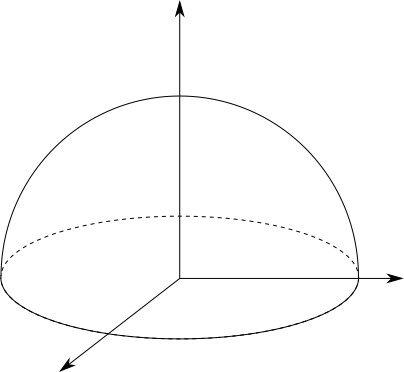
\includegraphics[width=0.5\textwidth]{hemisphere.svg}
%%     \caption{Upper hemisphere}
%%     \label{hemisphere}
%%   \end{figure}
%% }{
  \begin{figure}[H]
    \centering
    \def\svgwidth{0.5\columnwidth}
    \input{figures/latex/hemisphere.pdf_tex}
    \caption{Upper hemisphere}
    \label{hemisphere}
  \end{figure}
%% }
    
    Therefore in spherical coordinates, the limits will be given by
      \[
        0 \leq r \leq 2, \quad 0 \leq \varphi \leq \frac{\pi}{2}, \quad 0 \leq \theta \leq 2\pi.
      \]
    To express the integrand in spherical coordinates, we use
      \[
        x^2 + y^2 + z^2 = r^2 \text{ and } z = r\cos(\varphi).
      \]
    Thus we have
      \[
        z^2\sqrt{x^2 + y^2 + z^2} = r^2\cos^2(\varphi) \times \sqrt{r^2} = r^3\cos^2(\varphi).
      \]
    Hence the integral is
      \begin{align*}
        & \phantom{=} \int\nolimits_0^{2\pi} \int\nolimits_0^{\pi/2} \int\nolimits_0^2 \left(r^3\cos^2(\varphi)\right) \times \left(r^2\sin(\varphi)\right) \, dr \, d\varphi \, d\theta  \\
        & = \int\nolimits_0^{2\pi} \int\nolimits_0^{\pi/2} \int\nolimits_0^2 r^5\cos^2(\varphi)\sin(\varphi) \, dr \, d\varphi \, d\theta  \\
        & = \int\nolimits_0^{2\pi} \int\nolimits_0^{\pi/2} \left[\frac{1}{6}r^6\cos^2(\varphi)\sin(\varphi)\right]_0^2 \, d\varphi \, d\theta  \\
        & = \int\nolimits_0^{2\pi} \int\nolimits_0^{\pi/2} \frac{32}{3}\cos^2(\varphi)\sin(\varphi) \, d\varphi \, d\theta  \\
        & = \frac{32}{3} \int\nolimits_0^{2\pi} \left[-\frac{1}{3}\cos^3(\varphi)\right]_0^{\pi/2} \, d\theta  \\
        & = \frac{32}{9} \int\nolimits_0^{2\pi} \cos^3(0) - \cos^3\left(\frac{\pi}{2}\right) \, d\theta  \\
        & = \frac{32}{9} \int\nolimits_0^{2\pi} 1 \, d\theta  \\
        & = \frac{32}{9}\left[\theta\right]_0^{2\pi}  \\
        & = \frac{64}{9}\pi.
      \end{align*}
  \end{example}
  
  \subsubsection*{Surfaces given by constant values of $r$, $\theta$, $\varphi$}
  
  \begin{itemize}
    \item $r = a$, $a$ constant: sphere of radius $a$, centre at the origin.
    \item $\theta = \alpha$, $\alpha$ constant: half-plane perpendicular to the $(x, y)$-plane, bounded by the $z$-axis; $\alpha$ is the (anticlockwise) angle with the positive $x$-axis.
    \item $\varphi = \beta$, $\beta$ constant: varies depending on $\beta$.
      \begin{itemize}
        \item $\beta = 0$ gives the positive $z$-axis (not a surface).
        \item $0 < \beta < \dfrac{\pi}{2}$ gives a cone, centred around the positive $z$-axis, vertex at the origin; $\beta$ is the angle with the positive $z$-axis.
        \item $\beta = \dfrac{\pi}{2}$ gives the $(x, y)$-plane.
        \item $\dfrac{\pi}{\strut 2} < \beta < \pi$ gives a cone, centred around the negative $z$-axis, vertex at the origin; $\beta$ is the angle with the positive $z$-axis, so $\pi - \beta$ is the angle with the negative $z$-axis.
        \item $\beta = \pi$ gives the negative $z$-axis.
      \end{itemize}
  \end{itemize}
  
  Planes parallel to the $(x, y)$-plane are not given by constant functions in spherical coordinates (other than the $(x, y)$-plane itself).
  
  Consider a point the plane $z = a$, where $a$ is constant.  Then
    \[
      z = a = r\cos(\varphi),
    \]
  so, rearranging,
    \[
      r = \frac{a}{\cos(\varphi)} = a\sec(\varphi).
    \]
  
  For $0 \leq \varphi < \dfrac{\pi}{2}$, this gives the plane $z = a$.
  
  For $\dfrac{\pi}{2} < \varphi \leq \pi$, this gives the plane $z = - a$.
  
  \subsubsection*{Determining limits of regions in spherical coordinates}
  
  See the handout, distributed in the Wednesday Week 10 lecture, and also available on the Week 10 section of the course Moodle page.
  
  Note: this handout comes from a book (\emph{Calculus} by Anton, Bivens, and Davis), and uses $\rho$ in place of $r$ and $\phi$ in place of $\varphi$.
  
  \begin{example}
    Given a 3-dimensional region $G$, the triple integral
      \[
        \iiint_G 1 \, dV
      \]
    gives the volume of $G$.  (Often the $1$ is omitted.)  We will use this to derive the standard formula for the volume of a sphere.
    
    Let $G$ be a sphere of radius $a$, centred at the origin.  Then the volume $V$ of $G$ is
      \begin{align*}
        V = \iiint_G dV & = \int_0^{2\pi} \int_0^{\pi} \int_0^a r^2 \sin(\varphi) \, dr \, d\varphi \, d\theta  \\
        & = \int_0^{2\pi} \int_0^{\pi} \left[\frac{r^3}{3}\right] \sin(\varphi) \, d\varphi \, d\theta  \\
        & = \frac{a^3}{3} \int_0^{2\pi} \int_0^{\pi} \sin(\varphi) \, d\varphi \, d\theta  \\
        & = \frac{a^3}{3} \int_0^{2\pi} \left[- \cos(\varphi)\right]_0^{\pi} \, d\theta  \\
        & = \frac{a^3}{3} \int_0^{2\pi} 2 \, d\theta = \frac{4\pi a^3}{3}.
      \end{align*}
  \end{example}
  
  
    
  
  
% VOLUME is now just an example!
  
%  \subsection{Volume calculated as a triple integral}
%  
%  Consider a triple integral in which the integrand is $1$:
%    \[
%      \iiint_G 1 \, dV.
%    \]
%  This is often written simply as
%    \[
%      \iiint_G dV.
%    \]
%  What does this integral give us?  Consider the case when $G$ is a simple $xy$-solid:
%  
%  \begin{figure}[H]
%    \centering
%    \def\svgwidth{0.65\columnwidth}
%    \input{diagrams/tripleintegral3dregion.pdf_tex}
%  \end{figure}  
%  
%  with:
%    \begin{itemize}
%      \item lower surface $z = g_1(x, y)$;
%      \item upper surface $z = g_2(x, y)$;
%      \item projection $R$ onto the $(x, y)$-plane.
%    \end{itemize}
%  
%  Then
%    \begin{align*}
%      \iiint_G 1 \, dV & = \iint_R \left[\int\nolimits_{g_1(x, y)}^{g_2(x, y)} 1 \, dz\right] \, dA  \\
%      & = \iint_R \left[z\right]_{g_1(x, y)}^{g_2(x, y)} \, dA  \\
%      & = \iint_R g_2(x, y) - g_1(x, y) \, dA  \\
%      & = \underbrace{\iint_R g_2(x, y) \, dA}_{\text{volume under } g_2(x, y)} - \underbrace{\iint_R g_1(x, y) \, dA}_{\text{volume under } g_1(x, y)}.
%    \end{align*}
%    
%  Thus this triple integral gives the volume of the region $G$.
%    
%  In fact, this works for other regions, not just simple $xy$-solids.
%    
%  \subsubsection*{Alternative argument}
%    
%  Consider a solid $G$ with density given by $\delta(x, y, z)$ at a point $(x, y, z)$.  The mass $M$ of the solid is given by
%    \[
%      M = \iiint_G \delta(x, y, z) \, dV.
%    \]
%  (See Worksheet 9, question 3.)
%  
%  Suppose the density of $G$ is a constant $D$, and write $V$ for the volume of $G$.  Then
%    \[
%      D = \frac{M}{V}.
%    \]
%  If $D = 1$, this becomes
%    \[
%      1 = \frac{M}{V} = \frac{\iiint\limits_G 1 \, dV}{V}.
%    \]
%  Rearranging gives
%    \[
%      V = \iiint_G 1 \, dV.
%    \]
%  
%  \begin{examples} \ 
%  
%    \begin{enumerate}
%      \item Find the volume of the solid within the cylinder $x^2 + y^2 = 9$ and between the planes $z = 1$ and $x + z = 5$.
%      
%      Write $G$ for this solid.  It is a simple $xy$-solid, with lower surface $z = 1$ and upper surface $z = 5 - x$.  The projection of $G$ onto the $(x, y)$-plane is the circular region bounded by $x^2 + y^2 = 9$; we denote this region by $R$.  Hence the volume is
%        \begin{align*}
%          V = \iiint_G \, dV & = \iint_R \left[\int\nolimits_1^{5 - x} \, dz\right] \, dA  \\
%          & = \int\nolimits_{-3}^{3} \int\nolimits_{-\sqrt{9 - x^2}}^{\sqrt{9 - x^2}} \int\nolimits_1^{5 - x} \, dz \, dy \, dx  \\
%          & = \int\nolimits_{-3}^{3} \int\nolimits_{-\sqrt{9 - x^2}}^{\sqrt{9 - x^2}} \left[z\right]_1^{5 - x} \, dy \, dx  \\
%          & = \int\nolimits_{-3}^{3} \int\nolimits_{-\sqrt{9 - x^2}}^{\sqrt{9 - x^2}} 4 - x \, dy \, dx  \\
%          & = \int\nolimits_{-3}^{3} \left[(4 - x)y\right]_{-\sqrt{9 - x^2}}^{\sqrt{9 - x^2}} \, dx  \\
%          & = \int\nolimits_{-3}^{3} (8 - 2x)\sqrt{9 - x^2} \, dx  \\
%          & = 8\int\nolimits_{-3}^{3} \sqrt{9 - x^2} \, dx - \int\nolimits_{-3}^{3} 2x\sqrt{9 - x^2} \, dx  \\
%        \end{align*}
%      The first of these integrals with respect to $x$ could be calculated using the techniques for integrating functions involving square roots from Section~\ref{sect:sqrts}.  However, to make things simpler for us, observe that it is the area of the positive half of a circular disc of radius $3$ (centred at the origin).  Thus we have
%        \[
%          \int\nolimits_{-3}^{3} (8 - 2x)\sqrt{9 - x^2} \, dx = \frac{1}{2} \times 3^2 \pi = \frac{9}{2}\pi.
%        \]
%      For the second integral, it is straightforward to use a suitable substitution, but again, we can simplify the calculation by observing that the integrand,
%        \[
%          2x\sqrt{9 - x^2},
%        \]
%      is an odd function, and the interval of integration is $[-3, 3]$.  Thus this integral is $0$.  Hence the volume of the solid is
%        \[
%          V = 8\left(\frac{9}{2}\pi\right) - 0 = 36\pi.
%        \]
%      \item Find the volume of the solid $G$ bounded by the sphere $x^2 + y^2 + z^2 = 16$ and below by the cone $z = \sqrt{x^2 + y^2}$.
%      
%      The region $G$ is an ice-cream-cone-shaped solid cut from a sphere, so in this example we will use spherical coordinates.  In spherical coordinates, the equation of the sphere $x^2 + y^2 + z^2 = 16$ is $r = 4$, and the equation of the cone $z = \sqrt{x^2 + y^2}$ is
%        \begin{align*}
%          r\cos(\varphi) & = \sqrt{r^2\sin^2(\varphi)\cos^2(\theta) + r^2\sin^2(\varphi)\sin^2(\theta)}  \\
%          & = \sqrt{r^2\sin^2(\varphi)\left(\cos^2(\theta) + \sin^2(\theta)\right)}  \\
%          & = \sqrt{r^2\sin^2(\varphi)}  \\
%          & = r\sin(\varphi).
%        \end{align*}
%      Dividing both sides by $r\cos(\varphi)$ gives
%        \[
%          \tan(\varphi) = 1,
%        \]
%      so this cone is given by $\varphi = \dfrac{\pi}{4}$.  Using the \emph{Determination of Limits} handout to determine the limits for the triple integral, the volume of $G$ is given by
%        \begin{align*}
%          V = \iiint_G dV & = \int\nolimits_0^{2\pi} \int\nolimits_0^{\pi/4} \int\nolimits_0^4 r^2\sin(\varphi) \, dr \, d\varphi \, d\theta  \\
%          & = \int\nolimits_0^{2\pi} \int\nolimits_0^{\pi/4} \left[\frac{r^3}{3}\right]_0^4 \, d\varphi \, d\theta  \\
%          & = \int\nolimits_0^{2\pi} \int\nolimits_0^{\pi/4} \frac{64}{3}\sin{\varphi} \, d\varphi \, d\theta  \\
%          & = \frac{64}{3} \int\nolimits_0^{2\pi} \left[-\cos(\varphi)\right]_0^{\pi/4} \, d\theta  \\
%          & = \frac{64}{3} \int\nolimits_0^{2\pi} \left(1 - \frac{\sqrt{2}}{2}\right) \, d\theta  \\
%          & = \frac{64\pi}{3}(2 - \sqrt{2}).
%        \end{align*}
%    \end{enumerate}
%  \end{examples}
  
  
  
  
  
  
  
  
